% PCCSL 507 Machine Learning Lab - Complete Record (joined, double-side print order)
% Order: Exp1=marks, Exp2=dataframe, Exp3=sales, Exp4=hours, Exp5=MLR, Exp6=SLR California
\documentclass[11pt,twoside]{article}

\usepackage[paper=letterpaper,top=0.7in,bottom=0.63in,left=0.75in,right=0.75in,headheight=24pt,headsep=0.14in,footskip=0.38in]{geometry}

\usepackage[T1]{fontenc}
\usepackage{mathptmx} % Times clone
\usepackage{xcolor}
\definecolor{primary}{HTML}{1F3864}
\definecolor{greytext}{HTML}{555555}
\definecolor{gridgrey}{HTML}{999999}
\usepackage{fancyhdr}
\usepackage{array}
\usepackage{colortbl}
\usepackage{parskip}
\setlength{\parindent}{0pt}
\setlength{\parskip}{4pt}
\setlength{\abovedisplayskip}{4pt}
\setlength{\belowdisplayskip}{4pt}
\setlength{\abovedisplayshortskip}{2pt}
\setlength{\belowdisplayshortskip}{2pt}
\usepackage{graphicx}
\usepackage{amsmath}
\usepackage{listings}
\lstset{basicstyle=\large\ttfamily, breaklines=true, frame=single, showstringspaces=false}

\pagestyle{fancy}
\fancyhf{}
\fancyhead[C]{\textcolor{primary}{\textbf{\small PCCSL 508 Machine Learning Laboratory Record}}}
\renewcommand{\headrulewidth}{0.75pt}
\renewcommand{\headrule}{\hbox to\headwidth{\color{primary}\leaders\hrule height \headrulewidth\hfill}}
\fancyfoot[C]{\footnotesize DEPARTMENT OF CSE \hfill CAPE COLLEGE OF ENGINEERING ALAPPUZHA \hfill Page No. \thepage}
\renewcommand{\footrulewidth}{0pt}

\newcommand{\expheading}[1]{{\fontsize{14}{17}\selectfont\textbf{#1}\par}}
\newcommand{\fullrule}{\noindent\rule{\textwidth}{0.6pt}\par}
% Break to next odd (right-side) page; inserts an empty page only if needed
\newcommand{\tooddpage}{\clearpage\ifodd\value{page}\else\null\thispagestyle{empty}\newpage\fi}
\newcommand{\toevenpage}{\clearpage\ifodd\value{page}\null\thispagestyle{empty}\newpage\fi}

\begin{document}
\sloppy

% ================= COVER (p1) =================
\begin{center}
\vspace*{20pt}

\includegraphics[width=3.1cm]{cape_logo.jpg}\par
\vspace{10pt}
{\fontsize{15}{18}\selectfont\textcolor{primary}{\textbf{CAPE COLLEGE OF ENGINEERING ALAPPUZHA}}}\par
\vspace{10pt}
{\fontsize{11}{14}\selectfont Department of Computer Science and Engineering}\par
\vspace{28pt}
{\color{primary}\rule{\textwidth}{0.75pt}}\par
\vspace{6pt}
{\fontsize{20}{24}\selectfont\textcolor{primary}{\textbf{PCCSL 508 MACHINE LEARNING LAB}}}\par
\vspace{6pt}
{\color{primary}\rule{\textwidth}{0.75pt}}\par
\vspace{10pt}
{\fontsize{15}{18}\selectfont\textbf{LABORATORY RECORD}}\par
\vspace{28pt}
{\fontsize{11}{14}\selectfont Submitted by}\par
\vspace{8pt}
\end{center}

{\fontsize{11}{16}\selectfont
\begin{center}
\renewcommand{\arraystretch}{1.6}
\begin{tabular}{@{}p{3.6cm}@{\hspace{0.2cm}:\hspace{0.3cm}}l@{}}
Name & Goutham Sankar JL \\
Reg.\ No. & PRP24CS068 \\
Programme & B.Tech \\
Semester / Year & S5 \\
Academic Year & 2026-2027 \\
Faculty In-Charge & Ms. Sneha S, Ms. Deepa A B \\
\end{tabular}
\end{center}
\vspace{14pt}
\begin{center}
\begin{tabular}{@{}l@{\hspace{0.2cm}:\hspace{0.3cm}}l@{\hspace{1.0cm}}l@{\hspace{0.2cm}:\hspace{0.3cm}}l@{}}
Signature & \underline{\hspace{2.9cm}} & Date & \underline{\hspace{2.9cm}} \\
\end{tabular}
\end{center}
}

\tooddpage % p2 blank

% ================= INDEX (p3) =================
\begin{center}
{\fontsize{16}{19}\selectfont\textcolor{primary}{\textbf{INDEX}}}\par
\vspace{8pt}
\end{center}

\setlength{\tabcolsep}{4pt}
\arrayrulecolor{gridgrey}
\setlength{\arrayrulewidth}{0.5pt}
\noindent
\begin{tabular}{|>{\centering\arraybackslash}p{0.44in}|>{\centering\arraybackslash}p{3.34in}|>{\centering\arraybackslash}p{0.94in}|>{\centering\arraybackslash}p{0.75in}|>{\centering\arraybackslash}p{0.86in}|}
\hline
\rowcolor{primary}
\textcolor{white}{\textbf{\small Sl.\ No.}} & \textcolor{white}{\textbf{\small Title of the Experiment}} & \textcolor{white}{\textbf{\small Date}} & \textcolor{white}{\textbf{\small Page No.}} & \textcolor{white}{\textbf{\small Signature}} \\
\hline
1A & NumPy Basics -- Student Marks Analysis & 7-7-2026 & 5 & \\[14pt] \hline
1B & Pandas DataFrame -- Student Details & 7-7-2026 & 11 & \\[14pt] \hline
2 & NumPy 2D Array -- Branch Sales Analysis & 15-7-2026 & 17 & \\[14pt] \hline
3A & Simple Linear Regression -- Study Hours & 22-7-2026 & 25 & \\[14pt] \hline
3B & Multiple Linear Regression -- House Price & 22-7-2026 & 31 & \\[14pt] \hline
4A & Simple Linear Regression (Least Squares) & 14-8-2026 & 37 & \\[14pt] \hline
4B & Simple Linear Regression (Gradient Descent) & 14-8-2026 & 43 & \\[14pt] \hline
4C & Simple Linear Regression with Scikit-learn & 14-8-2026 & 51 & \\[14pt] \hline
5 & K-Nearest Neighbors on Breast Cancer & 9-9-2026 & 57 & \\[14pt] \hline
6 & Decision Tree on Online Retail & 9-9-2026 & 63 & \\[14pt] \hline
7 & Logistic Regression with and without Feature Scaling & 07-10-2026 & 71 & \\[14pt] \hline
8 & Ridge and Lasso Regularization & 07-10-2026 & 77 & \\[14pt] \hline
9 & Logistic Regression using MLE and MAP & 14-10-2026 & 85 & \\[14pt] \hline
10 & K-Means Clustering on Digits Dataset & 14-10-2026 & 91 & \\[14pt] \hline
11 & Multilayer Feed-Forward Neural Network (MLP) on Wine Quality Dataset using Keras & 30-10-2026 & 97 & \\[14pt] \hline
\end{tabular}

\tooddpage % p4 blank

% ============================================================
% EXPERIMENT 1 : NumPy marks (was standalone Exp 2)
% ============================================================
{\setlength{\parskip}{1pt}\setlength{\abovedisplayskip}{2pt}\setlength{\belowdisplayskip}{2pt}
\begin{center}
\expheading{EXPERIMENT NO. 1A}
\end{center}
\vspace{2pt}

\noindent\textbf{Date:} 7-7-2026\par
\vspace{6pt}

\expheading{TITLE}
\vspace{4pt}
\noindent NumPy Basics -- Student Marks Analysis\par
\vspace{4pt}

\expheading{AIM}
\vspace{4pt}
\noindent To store the marks of 3 students in 5 subjects in a NumPy array and compute the total, average, highest score and subject-wise average. \par
\vspace{4pt}

\expheading{OBJECTIVE}
\vspace{2pt}
\fullrule
\vspace{4pt}
\noindent To familiarize with NumPy array equations by storing the marks of 3 students in 5 subjects and finding the total, average, highest score and subject-wise average. \par
\vspace{4pt}

\expheading{THEORY}
\vspace{4pt}
Marks matrix ($3$ students $\times$ $5$ subjects):
\[M=\begin{bmatrix}m_{11} & \cdots & m_{15}\\m_{21} & \cdots & m_{25}\\m_{31} & \cdots & m_{35}\end{bmatrix}\]
Total of all marks:
\[T=\sum_{i=1}^{3}\sum_{j=1}^{5}m_{ij}\qquad\text{(np.sum)}\]
Overall average:
\[\bar{A}=\frac{T}{15}\qquad\text{(np.mean)}\]
Highest score and its position:
\[H=\max(M)\qquad\text{(np.max, np.argmax)}\]
Student-wise total (row sum, axis=1):
\[T_i=\sum_{j=1}^{5}m_{ij}\]
Subject-wise average (column mean, axis=0):
\[\bar{S}_j=\frac{1}{3}\sum_{i=1}^{3}m_{ij}\]
\vspace{4pt}

\expheading{PROCEDURE}
\vspace{4pt}
\noindent 1. Store the marks of 3 students in 5 subjects in a $3\times5$ NumPy array.\par
\noindent 2. Find the total (np.sum) and the average (np.mean) of all marks.\par
\noindent 3. Find the highest score (np.max) and its student/subject (np.argmax).\par
\noindent 4. Find the student-wise total (sum, axis=1) and subject-wise average (mean, axis=0).\par
\noindent 5. Display all results and verify them. \par
\vspace{4pt}

\expheading{DATASET DESCRIPTION}
\vspace{4pt}
\noindent Dataset Name: Student marks (synthetic, entered in program)\par
\noindent Source: 3 students $\times$ 5 subjects, marks out of 100\par
\noindent Number of Samples: 15 marks \hspace{0.3cm} Number of Features: 5 subjects\par
\noindent Target / Class: Not applicable (descriptive statistics)\par
\noindent Description: S1=[78, 85, 92, 88, 76]; S2=[65, 72, 80, 69, 74]; S3=[90, 88, 95, 91, 89]. \par
\vspace{4pt}
} % end sheet-local tightening

\toevenpage
\expheading{PROGRAM}
\vspace{6pt}

\begin{lstlisting}
import numpy as np


marks = np.array([
    [78, 85, 92, 88, 76],
    [65, 72, 80, 69, 74],
    [90, 88, 95, 91, 89],
])
print("Marks (3 students x 5 subjects):")
print(marks)

total = marks.sum()
average = marks.mean()
highest = marks.max()
pos = np.unravel_index(marks.argmax(), marks.shape)
print("Total =", total)
print("Average =", round(float(average), 2))
print("Highest score =", highest, "by student", pos[0] + 1,
      "in subject", pos[1] + 1)

stud_total = marks.sum(axis=1)
print("Student-wise total =", stud_total)
sub_avg = marks.mean(axis=0)
print("Subject-wise average =", np.round(sub_avg, 2))
\end{lstlisting}

\toevenpage
\expheading{OUTPUT}
\vspace{2pt}
\noindent\rule{\textwidth}{0.5pt}\par
\vspace{4pt}
\begin{verbatim}
Marks (3 students x 5 subjects):
[[78 85 92 88 76]
 [65 72 80 69 74]
 [90 88 95 91 89]]
Total = 1232
Average = 82.13
Highest score = 95 by student 3 in subject 3
Student-wise total = [419 360 453]
Subject-wise average = [77.67 81.67 89.   82.67 79.67]
\end{verbatim}
\vspace{4pt}

\tooddpage
\expheading{RESULT}
\vspace{4pt}
{\fontsize{12}{15}\selectfont
The above program was implemented and executed successfully using Python, and the corresponding output was obtained and verified. The results of the \textbf{NumPy array statistics} were analyzed and found to be satisfactory, thereby achieving the desired objective of the experiment.\par
}

\vspace{12pt}

\noindent\textbf{Faculty Signature:} \underline{\hspace{3.6cm}} \hfill \textbf{Date:} \underline{\hspace{2.8cm}}\par

\tooddpage

% ============================================================
% EXPERIMENT 2 : Pandas dataframe (was standalone Exp 3)
% ============================================================
{\setlength{\parskip}{1pt}\setlength{\abovedisplayskip}{2pt}\setlength{\belowdisplayskip}{2pt}
\begin{center}
\expheading{EXPERIMENT NO. 1B}
\end{center}
\vspace{2pt}

\noindent\textbf{Date:} 7-7-2026\par
\vspace{6pt}

\expheading{TITLE}
\vspace{4pt}
\noindent Pandas DataFrame -- Student Details\par
\vspace{4pt}

\expheading{AIM}
\vspace{4pt}
\noindent To create a student dataframe, display rows/columns, filter rows, compute summary statistics with department-wise average, and save it as CSV. \par
\vspace{4pt}

\expheading{OBJECTIVE}
\vspace{2pt}
\fullrule
\vspace{4pt}
\noindent To work with a Pandas DataFrame of five students (roll no, name, department, marks) and perform selection, filtering, aggregation and CSV export operations. \par
\vspace{4pt}

\expheading{THEORY}
\vspace{4pt}
DataFrame with rows and named columns:
\[\text{df}=\text{pd.DataFrame}(\{\text{columns}\})\qquad\text{df.head}(n),\; \text{df.tail}(n)\]
Column selection and boolean filtering:
\[\text{df}[[\text{``Name''},\text{``Marks''}]]\qquad \text{df}[\text{df}[\text{``Marks''}]>80]\]
Summary statistics:
\[\max,\; \min,\; \text{mean}=\frac{1}{n}\sum x_i,\; \text{sum}=\sum x_i\]
Department-wise average and CSV export:
\[\text{df.groupby}(\text{``Department''})[\text{``Marks''}].\text{mean}()\qquad \text{df.to\_csv}(\text{file})\]
\vspace{4pt}

\expheading{PROCEDURE}
\vspace{4pt}
\noindent 1. Create a DataFrame of 5 students with Roll no, Name, Department, Marks and display it.\par
\noindent 2. Display the first 3 rows (head), last 2 rows (tail) and only Name/Marks columns.\par
\noindent 3. Filter students with marks above 80 and students of CSE department.\par
\noindent 4. Compute highest, lowest, average and total marks; average mark department-wise.\par
\noindent 5. Save the DataFrame to CSV and verify the file. \par
\vspace{4pt}

\expheading{DATASET DESCRIPTION}
\vspace{4pt}
\noindent Dataset Name: Student details (entered in program)\par
\noindent Source: 5 students; departments CSE, ECE, ME\par
\noindent Number of Samples: 5 rows \hspace{0.3cm} Number of Features: 4 columns\par
\noindent Target / Class: Not applicable (data handling operations)\par
\noindent Description: Marks range 68--90; exported to exp3\_students.csv. \par
\vspace{4pt}
} % end sheet-local tightening

\toevenpage
\expheading{PROGRAM}
\vspace{6pt}

\begin{lstlisting}
import pandas as pd


data = {
    "Roll no": [1, 2, 3, 4, 5],
    "Name": ["Anu", "Ravi", "Meera", "Arjun", "Divya"],
    "Department": ["CSE", "ECE", "CSE", "ME", "CSE"],
    "Marks": [85, 72, 90, 68, 78],
}
df = pd.DataFrame(data)
print("Dataframe:")
print(df.to_string(index=False))

print("\nFirst 3 rows:")
print(df.head(3).to_string(index=False))
print("\nLast two rows:")
print(df.tail(2).to_string(index=False))
print("\nName and Marks columns:")
print(df[["Name", "Marks"]].to_string(index=False))
print("\nMarks more than 80:")
print(df[df["Marks"] > 80].to_string(index=False))
print("\nCSE department:")
print(df[df["Department"] == "CSE"].to_string(index=False))
print("\nHighest =", df["Marks"].max(), " Lowest =", df["Marks"].min(),
      " Avg =", round(df["Marks"].mean(), 2), " Total =", df["Marks"].sum())
print("\nAverage mark department wise:")
print(df.groupby("Department")["Marks"].mean().round(2).to_string())

df.to_csv("exp3_students.csv", index=False)
print("\nSaved to exp3_students.csv")
\end{lstlisting}

\toevenpage
\expheading{OUTPUT}
\vspace{2pt}
\noindent\rule{\textwidth}{0.5pt}\par
\vspace{4pt}
{\scriptsize
\begin{verbatim}
Dataframe:
 Roll no  Name Department  Marks
       1   Anu        CSE     85
       2  Ravi        ECE     72
       3 Meera        CSE     90
       4 Arjun         ME     68
       5 Divya        CSE     78

First 3 rows:
 Roll no  Name Department  Marks
       1   Anu        CSE     85
       2  Ravi        ECE     72
       3 Meera        CSE     90

Last two rows:
 Roll no  Name Department  Marks
       4 Arjun         ME     68
       5 Divya        CSE     78

Name and Marks columns:
 Name  Marks
  Anu     85
 Ravi     72
Meera     90
Arjun     68
Divya     78

Marks more than 80:
 Roll no  Name Department  Marks
       1   Anu        CSE     85
       3 Meera        CSE     90

CSE department:
 Roll no  Name Department  Marks
       1   Anu        CSE     85
       3 Meera        CSE     90
       5 Divya        CSE     78

Highest = 90  Lowest = 68  Avg = 78.6  Total = 393

Average mark department wise:
Department
CSE    84.33
ECE    72.00
ME     68.00

Saved to exp3_students.csv
\end{verbatim}}
\vspace{4pt}

\tooddpage
\expheading{RESULT}
\vspace{4pt}
{\fontsize{12}{15}\selectfont
The above program was implemented and executed successfully using Python, and the corresponding output was obtained and verified. The results of the \textbf{Pandas DataFrame operations} were analyzed and found to be satisfactory, thereby achieving the desired objective of the experiment.\par
}

\vspace{12pt}

\noindent\textbf{Faculty Signature:} \underline{\hspace{3.6cm}} \hfill \textbf{Date:} \underline{\hspace{2.8cm}}\par

\tooddpage

% ============================================================
% EXPERIMENT 3 : NumPy sales (was standalone Exp 4)
% ============================================================
{\setlength{\parskip}{1pt}\setlength{\abovedisplayskip}{2pt}\setlength{\belowdisplayskip}{2pt}
\begin{center}
\expheading{EXPERIMENT NO. 2}
\end{center}
\vspace{2pt}

\noindent\textbf{Date:} 15-7-2026\par
\vspace{6pt}

\expheading{TITLE}
\vspace{4pt}
\noindent NumPy 2D Array -- Branch Sales Analysis\par
\vspace{4pt}

\expheading{AIM}
\vspace{4pt}
\noindent To store sales data in a 2D array and compute branch/day-wise totals, averages and the highest-selling branch using NumPy. \par
\vspace{4pt}

\expheading{OBJECTIVE}
\vspace{2pt}
\fullrule
\vspace{4pt}
\noindent To use a 2D NumPy array for branch sales data and perform indexing, slicing and visualization to find weekly totals, branch averages, day-wise totals and the top branch. \par
\vspace{4pt}

\expheading{THEORY}
\vspace{4pt}
Sales matrix ($3$ branches $\times$ $7$ days):
\[S=\begin{bmatrix}s_{11} & \cdots & s_{17}\\s_{21} & \cdots & s_{27}\\s_{31} & \cdots & s_{37}\end{bmatrix}\]
Indexing and slicing:
\[S[0],\; S[1,3:],\; S[:,0:3]\]
Weekly total per branch and grand total:
\[W_i=\sum_{j=1}^{7}s_{ij}\quad(\text{axis}=1)\qquad T=\sum_{i,j}s_{ij}\]
Branch average and day-wise total:
\[\bar{B}_i=\frac{1}{7}\sum_{j=1}^{7}s_{ij}\qquad D_j=\sum_{i=1}^{3}s_{ij}\quad(\text{axis}=0)\]
Top branch:
\[k=\arg\max_i W_i\]
\vspace{4pt}

\expheading{PROCEDURE}
\vspace{4pt}
\noindent 1. Store the sales data of 3 branches over 7 days in a 2D NumPy array and display it.\par
\noindent 2. Display the 1st branch sales, Mon--Wed sales and 2nd-branch sales from Thursday.\par
\noindent 3. Find weekly total per branch, grand total, branch-wise average and day-wise total.\par
\noindent 4. Find the branch with the highest sales, display all results and plot the daily-sales bar, pie, line and scatter charts. \par
\vspace{4pt}

\expheading{DATASET DESCRIPTION}
\vspace{4pt}
\noindent Dataset Name: Branch sales (entered in program)\par
\noindent Source: 3 branches $\times$ 7 days (Mon--Sun), synthetic figures\par
\noindent Number of Samples: 21 entries \hspace{0.3cm} Number of Features: 7 days\par
\noindent Target / Class: Not applicable (aggregation operations)\par
\noindent Description: B1=[1200, 1350, 1100, 1450, 1600, 2000, 1800]; B2=[900, 1100, 950, 1200, 1300, 1700, 1500]; B3=[1500, 1600, 1400, 1750, 1900, 2200, 2100]. \par
\vspace{4pt}
} % end sheet-local tightening

\toevenpage
\expheading{PROGRAM}
\vspace{6pt}

\begin{lstlisting}
import numpy as np
import matplotlib
matplotlib.use("Agg")
import matplotlib.pyplot as plt

days = ["Mon", "Tue", "Wed", "Thu", "Fri", "Sat", "Sun"]

sales = np.array([
    [1200, 1350, 1100, 1450, 1600, 2000, 1800],
    [900, 1100, 950, 1200, 1300, 1700, 1500],
    [1500, 1600, 1400, 1750, 1900, 2200, 2100],
])

print("Complete sales data (branches x days):")
print(sales)

print("1st branch sales =", sales[0])

print("Mon-Wed sales:")
print(sales[:, 0:3])

print("2nd branch from Thursday =", sales[1, 3:])

print("Weekly total per branch =", sales.sum(axis=1))
print("Grand total =", sales.sum())

print("Branch-wise average =", np.round(sales.mean(axis=1), 2))

print("Day-wise total =", sales.sum(axis=0))

top = int(sales.sum(axis=1).argmax())
print("Highest sales: branch", top + 1)
\end{lstlisting}

\toevenpage
\expheading{PROGRAM (continued)}
\vspace{6pt}

\begin{lstlisting}
x = np.arange(len(days))
w = 0.25
plt.figure(figsize=(7, 4.5))
plt.bar(x - w, sales[0], width=w, label="Branch 1")
plt.bar(x, sales[1], width=w, label="Branch 2")
plt.bar(x + w, sales[2], width=w, label="Branch 3")
plt.xticks(x, days)
plt.xlabel("Day"); plt.ylabel("Sales"); plt.title("Daily Sales per Branch")
plt.legend(); plt.tight_layout(); plt.savefig("exp4_sales.png", dpi=150)
plt.figure(figsize=(5, 4))
L = ["Branch 1", "Branch 2", "Branch 3"]
plt.pie(sales.sum(axis=1), labels=L, autopct="%1.1f%%")
plt.title("Branch Share of Total Sales"); plt.tight_layout()
plt.savefig("exp4_pie.png", dpi=150)
plt.figure(figsize=(7, 4.5))
plt.plot(days, sales.sum(axis=0), marker="o", linewidth=2)
plt.xlabel("Day"); plt.ylabel("Total sales")
plt.title("Day-wise Total Sales Trend")
plt.tight_layout(); plt.savefig("exp4_line.png", dpi=150)
plt.figure(figsize=(7, 4.5))
plt.scatter(range(7), sales[0], s=40, label="Branch 1")
plt.scatter(range(7), sales[1], s=40, label="Branch 2")
plt.scatter(range(7), sales[2], s=40, label="Branch 3")
plt.xlabel("Day index"); plt.ylabel("Sales"); plt.title("Daily Sales Scatter per Branch")
plt.legend(); plt.tight_layout(); plt.savefig("exp4_scatter.png", dpi=150)
\end{lstlisting}

\toevenpage
\expheading{OUTPUT}
\vspace{2pt}
\noindent\rule{\textwidth}{0.5pt}\par
\vspace{4pt}
\begin{verbatim}
Complete sales data (branches x days):
[[1200 1350 1100 1450 1600 2000 1800]
 [ 900 1100  950 1200 1300 1700 1500]
 [1500 1600 1400 1750 1900 2200 2100]]
1st branch sales = [1200 1350 1100 1450 1600 2000 1800]
Mon-Wed sales:
[[1200 1350 1100]
 [ 900 1100  950]
 [1500 1600 1400]]
2nd branch from Thursday = [1200 1300 1700 1500]
Weekly total per branch = [10500  8650 12450]
Grand total = 31600
Branch-wise average = [1500.   1235.71 1778.57]
Day-wise total = [3600 4050 3450 4400 4800 5900 5400]
Highest sales: branch 3
\end{verbatim}
\vspace{4pt}

\begin{center}
\begin{minipage}{0.40\textwidth}\centering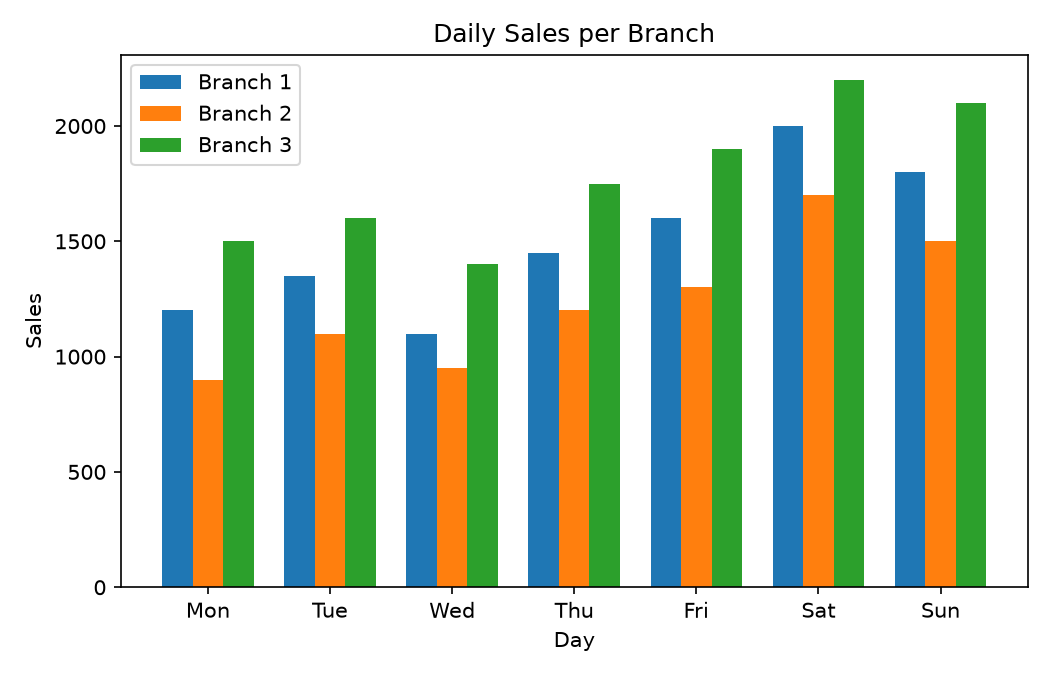
\includegraphics[width=\textwidth]{exp4_sales.png}\par{\small Fig. 1: Daily sales per branch.}\end{minipage}\hfill
\begin{minipage}{0.40\textwidth}\centering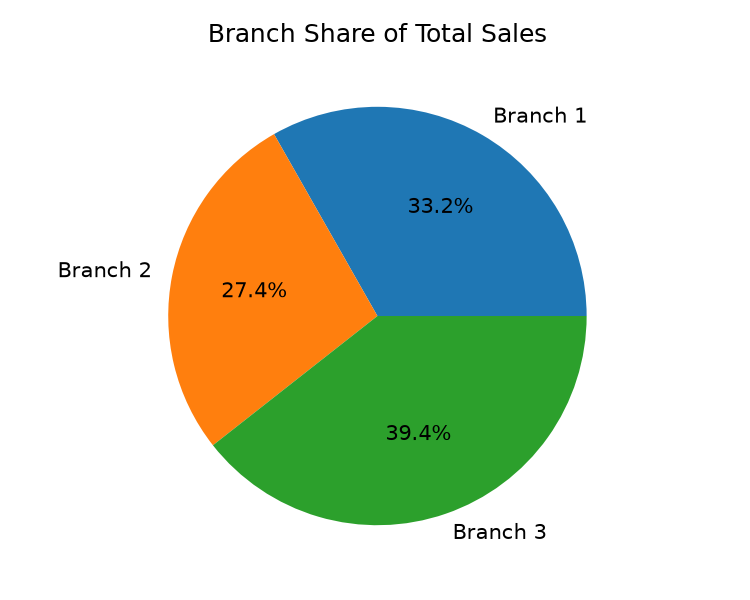
\includegraphics[width=\textwidth]{exp4_pie.png}\par{\small Fig. 2: Branch share of total sales.}\end{minipage}

\vspace{4pt}
\begin{minipage}{0.40\textwidth}\centering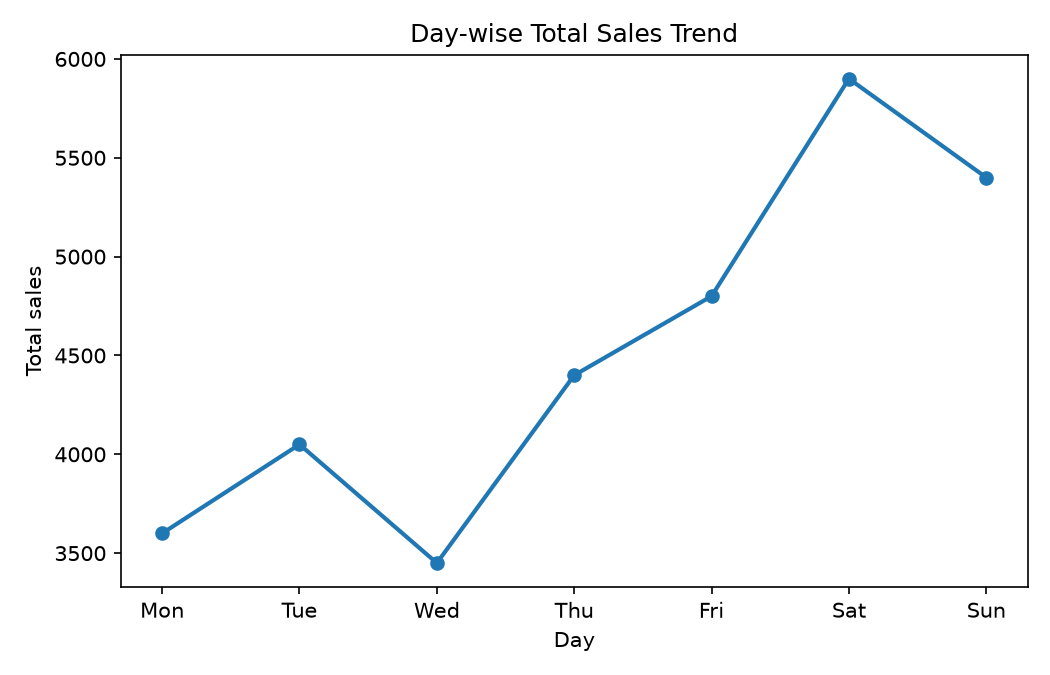
\includegraphics[width=\textwidth]{exp4_line.png}\par{\small Fig. 3: Day-wise total sales trend.}\end{minipage}\hfill
\begin{minipage}{0.40\textwidth}\centering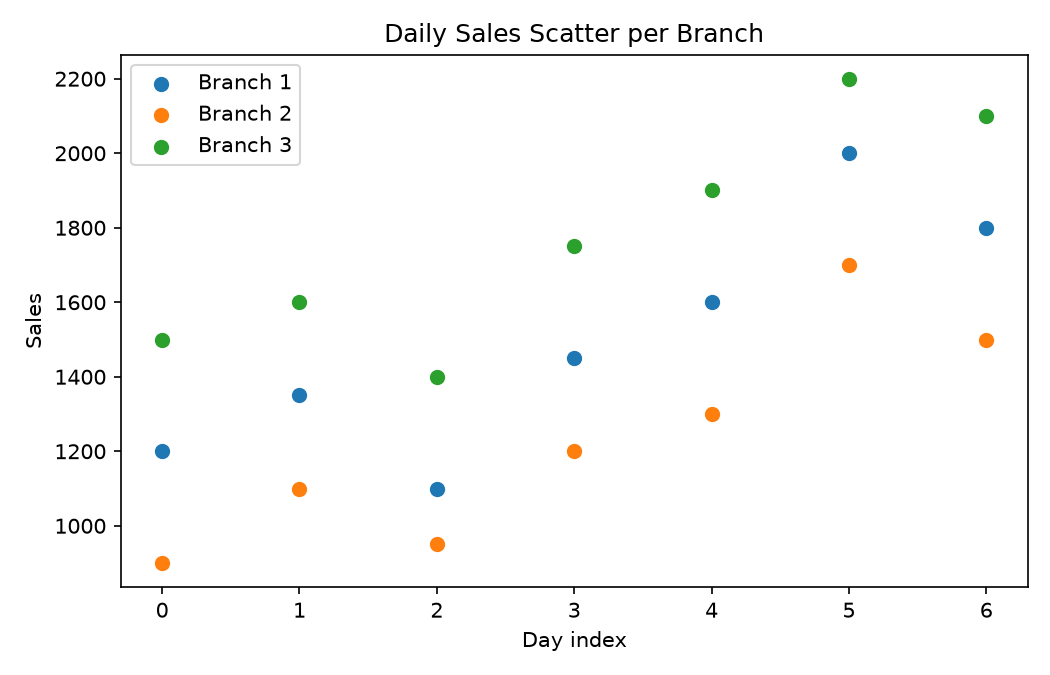
\includegraphics[width=\textwidth]{exp4_scatter.png}\par{\small Fig. 4: Daily sales scatter per branch.}\end{minipage}
\end{center}
\vspace{4pt}

\tooddpage
\expheading{RESULT}
\vspace{4pt}
{\fontsize{12}{15}\selectfont
The above program was implemented and executed successfully using Python, and the corresponding output was obtained and verified. The results of the \textbf{NumPy data visualization} were analyzed and found to be satisfactory, thereby achieving the desired objective of the experiment.\par
}

\vspace{12pt}

\noindent\textbf{Faculty Signature:} \underline{\hspace{3.6cm}} \hfill \textbf{Date:} \underline{\hspace{2.8cm}}\par

\tooddpage

% ============================================================
% EXPERIMENT 4 : SLR hours-score (was standalone Exp 5)
% ============================================================
{\setlength{\parskip}{1pt}\setlength{\abovedisplayskip}{2pt}\setlength{\belowdisplayskip}{2pt}
\begin{center}
\expheading{EXPERIMENT NO. 3A}
\end{center}
\vspace{2pt}

\noindent\textbf{Date:} 22-7-2026\par
\vspace{6pt}

\expheading{TITLE}
\vspace{4pt}
\noindent Simple Linear Regression -- Study Hours vs Exam Score\par
\vspace{4pt}

\expheading{AIM}
\vspace{4pt}
\noindent To fit $\hat{Y}=mX+b$ on hours-vs-score data with least squares and the normal equation, predict the 9-hour score, and evaluate with MSE and $R^2$. \par
\vspace{4pt}

\expheading{OBJECTIVE}
\vspace{2pt}
\fullrule
\vspace{4pt}
\noindent To implement simple linear regression on study-hours data by the regression equation and the standard (normal) equation, predict the score for 9 hours, and plot the regression line. \par
\vspace{4pt}

\expheading{THEORY}
\vspace{4pt}
Regression equation:
\[\hat{Y}=mX+b\]
Least-squares estimates:
\[m=\frac{\sum_{i=1}^{n}(X_i-\bar{X})(Y_i-\bar{Y})}{\sum_{i=1}^{n}(X_i-\bar{X})^2}\qquad b=\bar{Y}-m\bar{X}\]
Prediction and goodness of fit:
\[\hat{Y}(9)=m\cdot9+b\qquad \mathrm{MSE}=\frac{1}{n}\sum(Y_i-\hat{Y}_i)^2\qquad R^2=1-\frac{\sum(Y_i-\hat{Y}_i)^2}{\sum(Y_i-\bar{Y})^2}\]
\vspace{4pt}

\expheading{PROCEDURE}
\vspace{4pt}
\noindent 1. Store hours (X) and scores (Y) of 8 students in NumPy arrays.\par
\noindent 2. Compute $m,b$ by least squares and by the normal equation.\par
\noindent 3. Predict the score for 9 study hours with both equations.\par
\noindent 4. Compute MSE and $R^2$; plot data points with the regression line. \par
\vspace{4pt}

\expheading{DATASET DESCRIPTION}
\vspace{4pt}
\noindent Dataset Name: Study hours vs exam score (given table)\par
\noindent Source: 8 students; X = hours (1--8), Y = score out of 100\par
\noindent Number of Samples: 8 \hspace{0.3cm} Number of Features: 1 (hours)\par
\noindent Target / Class: Exam score (0--100)\par
\noindent Description: Y = [45, 50, 54, 60, 65, 70, 74, 80]; predict at X = 9. \par
\vspace{4pt}
} % end sheet-local tightening

\toevenpage
\expheading{PROGRAM}
\vspace{6pt}

\begin{lstlisting}
import numpy as np
import matplotlib
matplotlib.use("Agg")
import matplotlib.pyplot as plt


X = np.array([1, 2, 3, 4, 5, 6, 7, 8], dtype=float)
Y = np.array([45, 50, 54, 60, 65, 70, 74, 80], dtype=float)


x_bar, y_bar = X.mean(), Y.mean()
m = ((X - x_bar) * (Y - y_bar)).sum() / ((X - x_bar) ** 2).sum()
b = y_bar - m * x_bar
print(f"Least squares: m = {m:.4f}  b = {b:.4f}")


Xb = np.c_[np.ones(len(X)), X]
t = np.linalg.inv(Xb.T @ Xb) @ Xb.T @ Y
print(f"Normal equation: b = {t[0]:.4f}  m = {t[1]:.4f}")


print(f"LS prediction for 9 hrs = {m * 9 + b:.2f}")
print(f"NE prediction for 9 hrs = {t[1] * 9 + t[0]:.2f}")


for nm, (mm, bb) in [("LS", (m, b)), ("NE", (t[1], t[0]))]:
    p = mm * X + bb
    mse = float(((Y - p) ** 2).mean())
    r2 = float(1 - ((Y - p) ** 2).sum() / ((Y - y_bar) ** 2).sum())
    print(f"{nm}: MSE={mse:.4f} R2={r2:.4f}")


plt.figure(figsize=(7, 4.5))
plt.scatter(X, Y, s=40, label="Data points")
xs = np.linspace(0, 10, 200)
plt.plot(xs, m * xs + b, linewidth=2, label="Regression line")
plt.plot(9, m * 9 + b, marker="*", markersize=14, label="Prediction (9 hrs)")
plt.xlabel("Hours study (X)")
plt.ylabel("Exam score (Y)")
plt.title("Simple Linear Regression: Study Hours vs Exam Score")
plt.legend()
plt.tight_layout()
plt.savefig("exp5_fit.png", dpi=150)
\end{lstlisting}

\toevenpage
\expheading{OUTPUT}
\vspace{2pt}
\noindent\rule{\textwidth}{0.5pt}\par
\vspace{4pt}
\begin{verbatim}
Least squares: m = 4.9762  b = 39.8571
Normal equation: b = 39.8571  m = 4.9762
LS prediction for 9 hrs = 84.64
NE prediction for 9 hrs = 84.64
LS: MSE=0.1845 R2=0.9986
NE: MSE=0.1845 R2=0.9986
\end{verbatim}
\vspace{4pt}

\begin{center}
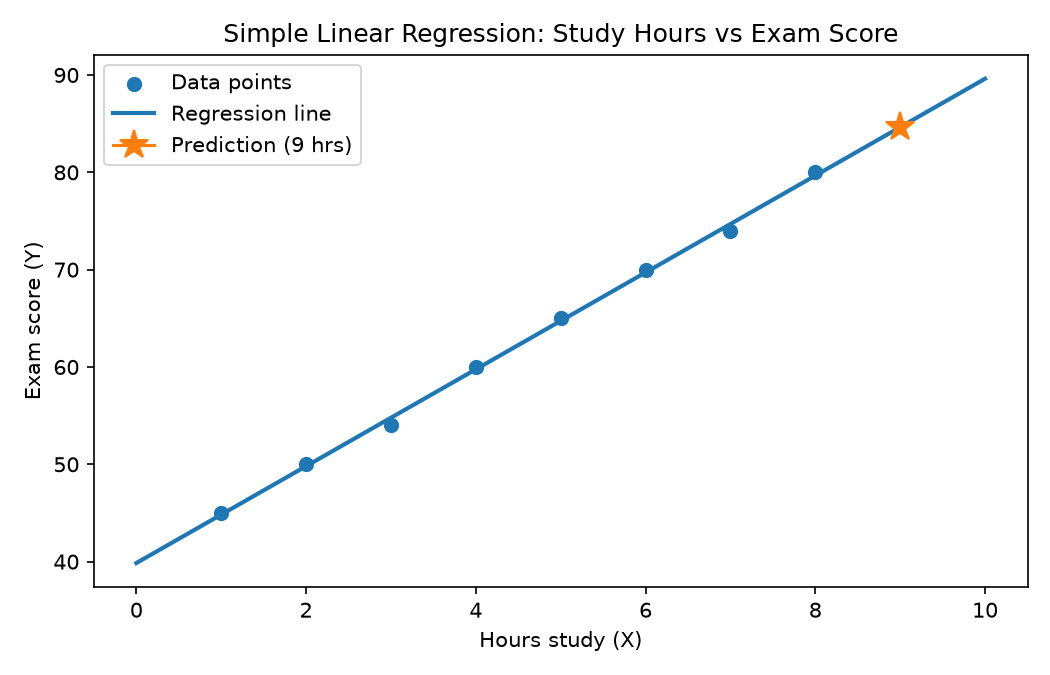
\includegraphics[width=0.78\textwidth]{exp5_fit.png}\par
\small Fig. 1: Data points, regression line and 9-hour prediction.\par
\end{center}
\vspace{4pt}

\tooddpage
\expheading{RESULT}
\vspace{4pt}
{\fontsize{12}{15}\selectfont
The above program was implemented and executed successfully using Python, and the corresponding output was obtained and verified. The results of the \textbf{least squares regression} were analyzed and found to be satisfactory, thereby achieving the desired objective of the experiment.\par
}

\vspace{12pt}

\noindent\textbf{Faculty Signature:} \underline{\hspace{3.6cm}} \hfill \textbf{Date:} \underline{\hspace{2.8cm}}\par

\tooddpage

% ============================================================
% EXPERIMENT 5 : MLR area-age (was standalone Exp 6)
% ============================================================
{\setlength{\parskip}{1pt}\setlength{\abovedisplayskip}{2pt}\setlength{\belowdisplayskip}{2pt}
\begin{center}
\expheading{EXPERIMENT NO. 3B}
\end{center}
\vspace{2pt}

\noindent\textbf{Date:} 22-7-2026\par
\vspace{6pt}

\expheading{TITLE}
\vspace{4pt}
\noindent Multiple Linear Regression -- House Price from Area and Age\par
\vspace{4pt}

\expheading{AIM}
\vspace{4pt}
\noindent To fit $\hat{Y}=b_0+b_1X_1+b_2X_2$ on the 6-house data, predict a new house price, and assess the fit. \par
\vspace{4pt}

\expheading{OBJECTIVE}
\vspace{2pt}
\fullrule
\vspace{4pt}
\noindent To predict house selling price from area and age using multiple linear regression with the normal equation, and evaluate it with MSE and R-squared with a 3D plot. \par
\vspace{4pt}

\expheading{THEORY}
\vspace{4pt}
Regression plane (two variables):
\[\hat{Y}=b_0+b_1X_1+b_2X_2\]
Normal equation with bias column $X=[\mathbf{1}\;X_1\;X_2]$:
\[\theta=(X^TX)^{-1}X^Ty,\qquad \theta=[b_0,b_1,b_2]^T\]
Prediction and goodness of fit:
\[\hat{Y}_{new}=b_0+b_1X_{1,new}+b_2X_{2,new}\qquad \mathrm{MSE}=\frac{1}{n}\sum(Y_i-\hat{Y}_i)^2\qquad R^2=1-\frac{\sum(Y_i-\hat{Y}_i)^2}{\sum(Y_i-\bar{Y})^2}\]
\vspace{4pt}

\expheading{PROCEDURE}
\vspace{4pt}
\noindent 1. Store Area ($X_1$), Age ($X_2$) and Price ($Y$) of 6 houses in NumPy arrays.\par
\noindent 2. Build $X$ with a bias column and solve $\theta=(X^TX)^{-1}X^Ty$.\par
\noindent 3. Predict the price of a new house (Area 2.8, Age 4).\par
\noindent 4. Compute MSE and $R^2$; plot houses with the fitted plane in 3D. \par
\vspace{4pt}

\expheading{DATASET DESCRIPTION}
\vspace{4pt}
\noindent Dataset Name: House price vs area and age (given table)\par
\noindent Source: 6 houses; $X_1$ = area, $X_2$ = age (years), $Y$ = price (lakhs)\par
\noindent Number of Samples: 6 \hspace{0.3cm} Number of Features: 2\par
\noindent Target / Class: Selling price in lakhs\par
\noindent Description: Area=[1.0--3.5]; Age=[10--2]; Price=[20--43]. \par
\vspace{4pt}
} % end sheet-local tightening

\toevenpage
\expheading{PROGRAM}
\vspace{6pt}

\begin{lstlisting}
import numpy as np
import matplotlib
matplotlib.use("Agg")
import matplotlib.pyplot as plt


X1 = np.array([1.0, 1.5, 2.0, 2.5, 3.0, 3.5])
X2 = np.array([10, 8, 6, 5, 3, 2], dtype=float)
Y = np.array([20, 24, 29, 32, 38, 43], dtype=float)


Xb = np.c_[np.ones(len(X1)), X1, X2]
t = np.linalg.inv(Xb.T @ Xb) @ Xb.T @ Y
b0, b1, b2 = t
print(f"Plane: Y = {b0:.4f} + {b1:.4f}*Area + {b2:.4f}*Age")


p = Xb @ t
mse = float(((Y - p) ** 2).mean())
r2 = float(1 - ((Y - p) ** 2).sum() / ((Y - Y.mean()) ** 2).sum())
print(f"MLR: MSE={mse:.4f} R2={r2:.4f} RMSE={np.sqrt(mse):.4f}")


new = b0 + b1 * 2.8 + b2 * 4
print(f"Predicted price (Area 2.8, Age 4) = {new:.2f} lakhs")


fig = plt.figure(figsize=(7, 5))
ax = fig.add_subplot(111, projection="3d")
ax.scatter(X1, X2, Y, s=40, label="Houses")
a = np.linspace(0.8, 3.7, 20)
g = np.linspace(1, 11, 20)
A, G = np.meshgrid(a, g)
ax.plot_surface(A, G, b0 + b1 * A + b2 * G, alpha=0.4)
ax.scatter([2.8], [4], [new], s=80, marker="*",
           label="Prediction (2.8, 4)")
ax.set_xlabel("Area X1")
ax.set_ylabel("Age X2")
ax.set_zlabel("Price Y (lakhs)")
ax.set_title("Multiple Linear Regression: Price vs Area and Age")
ax.legend()
plt.tight_layout()
plt.savefig("exp6_plane.png", dpi=150)
\end{lstlisting}

\toevenpage
\expheading{OUTPUT}
\vspace{2pt}
\noindent\rule{\textwidth}{0.5pt}\par
\vspace{4pt}
\begin{verbatim}
Plane: Y = 10.4286 + 9.1429*Area + 0.0000*Age
MLR: MSE=0.3810 R2=0.9938 RMSE=0.6172
Predicted price (Area 2.8, Age 4) = 36.03 lakhs
\end{verbatim}
\vspace{4pt}

\begin{center}
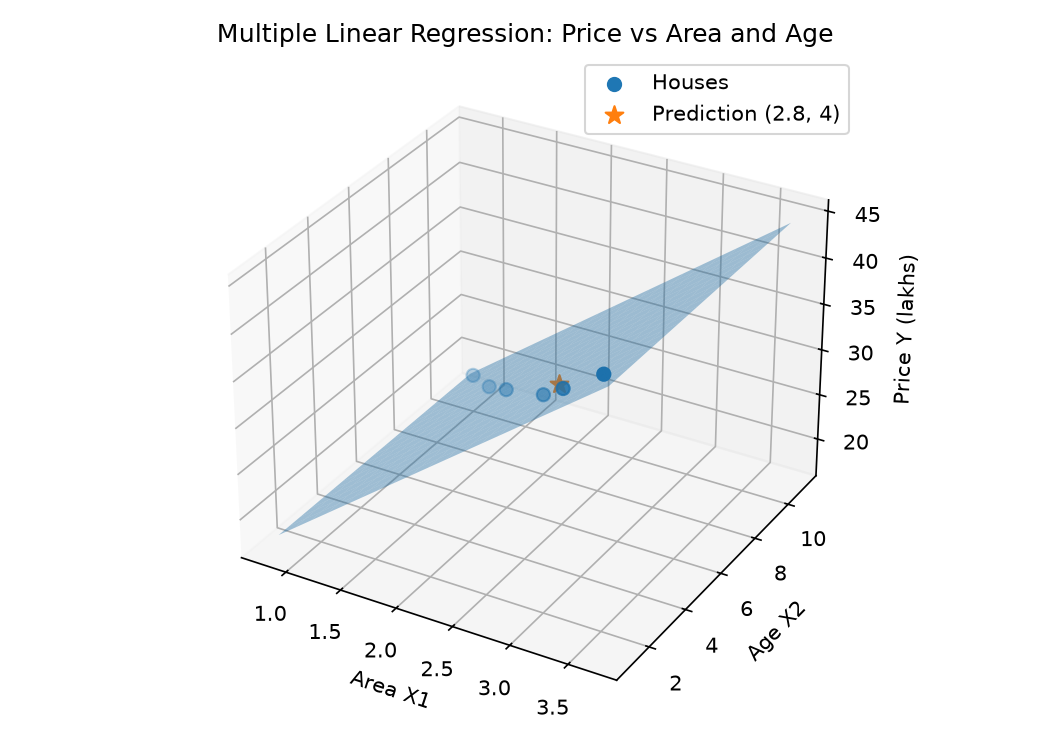
\includegraphics[width=0.78\textwidth]{exp6_plane.png}\par
\small Fig. 1: Houses, fitted plane and predicted house (star).\par
\end{center}
\vspace{4pt}

\tooddpage
\expheading{RESULT}
\vspace{4pt}
{\fontsize{12}{15}\selectfont
The above program was implemented and executed successfully using Python, and the corresponding output was obtained and verified. The results of the \textbf{multiple linear regression} were analyzed and found to be satisfactory, thereby achieving the desired objective of the experiment.\par
}

\vspace{12pt}

\noindent\textbf{Faculty Signature:} \underline{\hspace{3.6cm}} \hfill \textbf{Date:} \underline{\hspace{2.8cm}}\par

\tooddpage

% ============================================================
% EXPERIMENT 4A
% ============================================================
{\setlength{\parskip}{1pt}\setlength{\abovedisplayskip}{2pt}\setlength{\belowdisplayskip}{2pt}
\begin{center}
\expheading{EXPERIMENT NO. 4A}
\end{center}
\vspace{2pt}

\noindent\textbf{Date:} 14-8-2026\par
\vspace{6pt}

\expheading{TITLE}
\vspace{4pt}
\noindent Simple Linear Regression using Least Squares -- TotalRooms\par
\vspace{4pt}

\expheading{AIM}
\vspace{4pt}
\noindent To fit $\hat{Y}=mX+b$ by least squares on TotalRooms, predict test values, and assess the fit with MSE and $R^2$. \par
\vspace{4pt}

\expheading{OBJECTIVE}
\vspace{2pt}
\fullrule
\vspace{4pt}
\noindent To implement least squares regression on housing.csv (X=TotalRooms, Y=MedHouseVal) and evaluate it with MSE, R-squared and the regression-line plot. \par
\vspace{4pt}

\expheading{THEORY}
\vspace{4pt}
Regression equation:
\[\hat{Y}=mX+b\]
Least-squares estimates:
\[m=\frac{\sum_{i=1}^{n}(X_i-\bar{X})(Y_i-\bar{Y})}{\sum_{i=1}^{n}(X_i-\bar{X})^2}\qquad b=\bar{Y}-m\bar{X}\]
Goodness of fit:
\[\mathrm{MSE}=\frac{1}{n}\sum_{i=1}^{n}(Y_i-\hat{Y}_i)^2\qquad R^2=1-\frac{\sum_{i=1}^{n}(Y_i-\hat{Y}_i)^2}{\sum_{i=1}^{n}(Y_i-\bar{Y})^2}\]
\vspace{4pt}

\expheading{PROCEDURE}
\vspace{4pt}
\noindent 1. Load the California Housing dataset (housing.csv).\par
\noindent 2. Identify the variables: independent $X=$ TotalRooms (Total rooms); dependent $Y=$ MedHouseVal (Median House Value).\par
\noindent 3. Inspect the dataset for missing, duplicate, or invalid values.\par
\noindent 4. Calculate the slope $m$ and the intercept $b$ using the least square equation.\par
\noindent 5. Construct the regression equation $\hat{Y}=mX+b$.\par
\noindent 6. Use the regression equation to predict the target values for the test dataset.\par
\noindent 7. Calculate the Mean Squared Error (MSE) and the coefficient of determination $R^2$ to measure the goodness of fit.\par
\noindent 8. Plot the actual data points and regression line. \par
\vspace{4pt}

\expheading{DATASET DESCRIPTION}
\vspace{4pt}
\noindent Dataset Name: California Housing (housing.csv)\par
\noindent Source: Public census CSV file; prepared with NumPy only\par
\noindent Number of Samples: 20640 usable (0 missing) \hspace{0.3cm} Number of Features: 1 (TotalRooms)\par
\noindent Target / Class: MedHouseVal $-$ median house value in units of \$100{,}000\par
\noindent Description: Train 16512 / test 4128 (80/20, seed 42). \par
\vspace{4pt}
} % end sheet-local tightening
\toevenpage
\expheading{PROGRAM}
\vspace{6pt}

\begin{lstlisting}
import csv
import numpy as np
import matplotlib
matplotlib.use("Agg")
import matplotlib.pyplot as plt
rooms, prices, miss = [], [], 0
with open("housing.csv", newline="") as f:
    for r in csv.DictReader(f):
        try:
            rooms.append(float(r["total_rooms"]))
            prices.append(float(r["median_house_value"]))
        except (ValueError, KeyError):
            miss += 1
X = np.array(rooms)
y = np.array(prices) / 1e5
print("Usable:", len(X), " Missing:", miss)
rng = np.random.default_rng(42)
order = np.arange(len(X))
rng.shuffle(order)
n_train = int(0.8 * len(X))
X_train, X_test = X[order[:n_train]], X[order[n_train:]]
y_train, y_test = y[order[:n_train]], y[order[n_train:]]
print("Train:", len(X_train), " Test:", len(X_test))
x_bar = X_train.mean()
y_bar = y_train.mean()
m = ((X_train - x_bar) * (y_train - y_bar)).sum()
m = m / ((X_train - x_bar) ** 2).sum()
b = y_bar - m * x_bar
print(f"LS slope m = {m:.6f}")
print(f"LS intercept b = {b:.4f}")
y_pred = m * X_test + b
mse = ((y_test - y_pred) ** 2).mean()
r2 = 1 - ((y_test - y_pred) ** 2).sum() / ((y_test - y_test.mean()) ** 2).sum()
print(f"LS: MSE={mse:.4f} R2={r2:.4f} RMSE={np.sqrt(mse):.4f}")
plt.figure(figsize=(7, 4.5))
plt.scatter(X_test, y_test, s=6, alpha=0.25, label="Test data")
xs = np.linspace(0, float(np.percentile(X, 99.5)), 200)
plt.plot(xs, m * xs + b, linewidth=2, label="Least Squares line")
plt.xlabel("TotalRooms (X)")
plt.ylabel("MedHouseVal ($100k) (Y)")
plt.title("Simple Linear Regression (Least Squares): TotalRooms vs Price")
plt.legend()
plt.tight_layout()
plt.savefig("exp4a_fit.png", dpi=150)
\end{lstlisting}
\toevenpage
\expheading{OUTPUT}
\vspace{2pt}
\noindent\rule{\textwidth}{0.5pt}\par
\vspace{4pt}
\begin{verbatim}
Usable: 20640  Missing: 0
Train: 16512  Test: 4128
LS slope m = 0.000072
LS intercept b = 1.8840
LS: MSE=1.3236 R2=0.0167 RMSE=1.1505
\end{verbatim}
\vspace{4pt}

\begin{center}
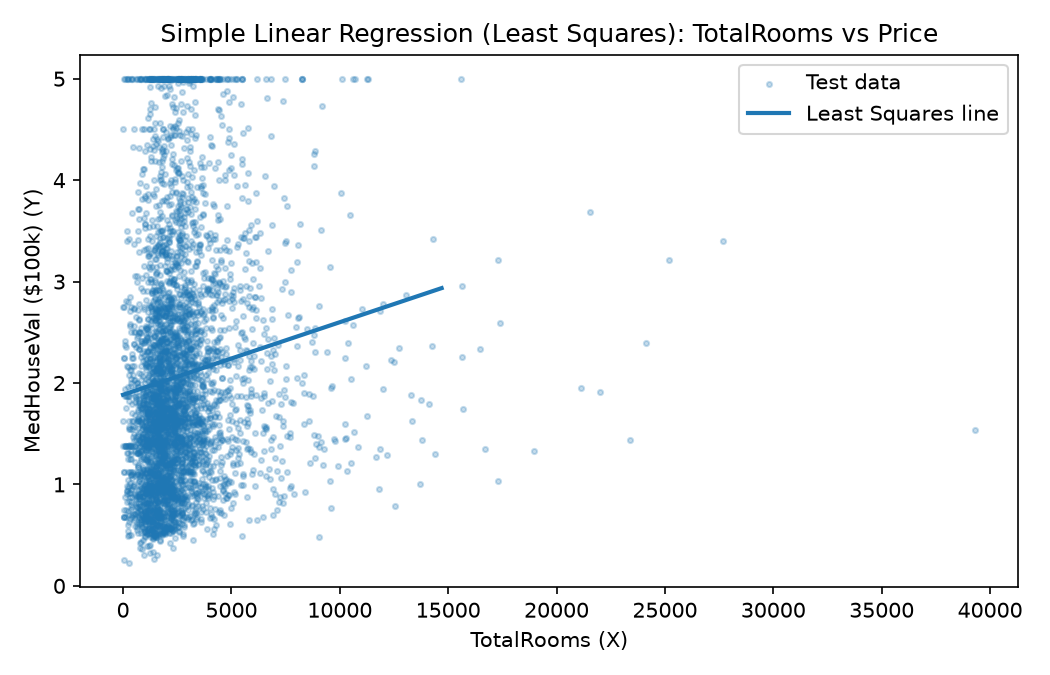
\includegraphics[width=0.78\textwidth]{exp4a_fit.png}\par
\small Fig. 1: Test data with the least-squares regression line.\par
\end{center}
\vspace{4pt}

\tooddpage
\expheading{RESULT}
\vspace{4pt}
{\fontsize{12}{15}\selectfont
The above program was implemented and executed successfully using Python, and the corresponding output was obtained and verified. The results of the \textbf{least squares regression} were analyzed and found to be satisfactory, thereby achieving the desired objective of the experiment.\par
}

\vspace{12pt}

\noindent\textbf{Faculty Signature:} \underline{\hspace{3.6cm}} \hfill \textbf{Date:} \underline{\hspace{2.8cm}}\par

\tooddpage

% ============================================================
% EXPERIMENT 4B
% ============================================================
{\setlength{\parskip}{0pt}\setlength{\abovedisplayskip}{0pt}\setlength{\belowdisplayskip}{0pt}
\begin{center}
\expheading{EXPERIMENT NO. 4B}
\end{center}
\vspace{2pt}

\noindent\textbf{Date:} 14-8-2026\par
\vspace{6pt}

\expheading{TITLE}
\vspace{4pt}
\noindent Simple Linear Regression using Gradient Descent -- TotalRooms\par
\vspace{4pt}

\expheading{AIM}
\vspace{4pt}
\noindent To fit $\hat{Y}=mX+b$ by gradient descent from $m=c=0$, predict test values, and assess with MSE and $R^2$. \par
\vspace{4pt}

\expheading{OBJECTIVE}
\vspace{2pt}
\fullrule
\vspace{4pt}
\noindent To implement gradient descent regression on housing.csv (X=TotalRooms, Y=MedHouseVal) with $\alpha=0.01$ and 100 epochs, and evaluate it with MSE, R-squared and the cost curve. \par
\vspace{4pt}

\expheading{THEORY}
\vspace{4pt}
Linear hypothesis:
\[\hat{Y}=mX+b\]
Mean Squared Error cost:
\[J(m,c)=\frac{1}{n}\sum_{i=1}^{n}(Y_i-\hat{Y}_i)^2\]
Gradients:
\[\frac{\partial J}{\partial m}=-\frac{2}{n}\sum_{i=1}^{n}X_i(Y_i-\hat{Y}_i)\qquad \frac{\partial J}{\partial b}=-\frac{2}{n}\sum_{i=1}^{n}(Y_i-\hat{Y}_i)\]
Gradient descent updates:
\[m:=m-\alpha\frac{\partial J}{\partial m}\qquad b:=b-\alpha\frac{\partial J}{\partial b}\]
\vspace{4pt}

\expheading{PROCEDURE}
\vspace{4pt}
\noindent 1. Load the California Housing dataset and select TotalRooms as $X$ and MedHouseVal as $Y$.\par
\noindent 2. Inspect and clean the data by checking missing and invalid values.\par
\noindent 3. Split the dataset into training and testing sets.\par
\noindent 4. Standardize the input feature using the mean and standard deviation of the training data.\par
\noindent 5. Initialize slope $m=0$ and intercept $c=0$.\par
\noindent 6. Choose learning rate $\alpha=0.01$ and epochs $=100$.\par
\noindent 7. Calculate the predicted values.\par
\noindent 8. Calculate the Mean Squared Error cost $J(m,c)=\frac{1}{n}\sum(Y_i-\hat{Y}_i)^2$.\par
\noindent 9. Calculate the gradient w.r.t.\ slope $\frac{\partial J}{\partial m}=-\frac{2}{n}\sum X_i(Y_i-\hat{Y}_i)$.\par
\noindent 10. Calculate the gradient w.r.t.\ intercept $\frac{\partial J}{\partial b}=-\frac{2}{n}\sum(Y_i-\hat{Y}_i)$.\par
\noindent 11. Update slope $m=m-\alpha\frac{\partial J}{\partial m}$ and intercept $b=b-\alpha\frac{\partial J}{\partial b}$.\par
\noindent 12. Repeat steps 8--11 for 100 epochs or until the cost converges.\par
\noindent 13. Plot cost versus epochs to verify convergence.\par
\noindent 14. Predict test values with final $m,b$; calculate MSE and $R^2$. \par
\vspace{4pt}

\expheading{DATASET DESCRIPTION}
\vspace{4pt}
\noindent Dataset Name: California Housing (housing.csv)\par
\noindent Source: Public census CSV file; prepared with NumPy only; feature standardized\par
\noindent Number of Samples: 20640 usable (0 missing) \hspace{0.3cm} Number of Features: 1 (TotalRooms)\par
\noindent Target / Class: MedHouseVal $-$ median house value in units of \$100{,}000\par
\noindent Description: Train 16512 / test 4128 (80/20, seed 42). \par
\vspace{4pt}
} % end sheet-local tightening
\toevenpage
\expheading{PROGRAM}
\vspace{6pt}

\begin{lstlisting}
import csv
import numpy as np
import matplotlib
matplotlib.use("Agg")
import matplotlib.pyplot as plt
rooms, prices, miss = [], [], 0
with open("housing.csv", newline="") as f:
    for r in csv.DictReader(f):
        try:
            rooms.append(float(r["total_rooms"]))
            prices.append(float(r["median_house_value"]))
        except (ValueError, KeyError):
            miss += 1
X = np.array(rooms)
y = np.array(prices) / 1e5
print("Usable:", len(X), " Missing:", miss)
rng = np.random.default_rng(42)
order = np.arange(len(X))
rng.shuffle(order)
n_train = int(0.8 * len(X))
X_train, X_test = X[order[:n_train]], X[order[n_train:]]
y_train, y_test = y[order[:n_train]], y[order[n_train:]]
print("Train:", len(X_train), " Test:", len(X_test))
mu = X_train.mean()
sg = X_train.std()
Xs_train = (X_train - mu) / sg
m, b = 0.0, 0.0
n = len(Xs_train)
costs = []
for epoch in range(100):
    y_hat = m * Xs_train + b
    err = y_train - y_hat
    J = (err ** 2).mean()
    costs.append(float(J))
    dm = (-2 / n) * (Xs_train * err).sum()
    db = (-2 / n) * err.sum()
    m = m - 0.01 * dm
    b = b - 0.01 * db
\end{lstlisting}

\toevenpage
\expheading{PROGRAM (continued)}
\vspace{6pt}

\begin{lstlisting}
m_gd = m / sg
b_gd = b - m * mu / sg
print(f"GD slope m = {m_gd:.6f}")
print(f"GD intercept b = {b_gd:.4f}")
print(f"GD cost first={costs[0]:.4f} last={costs[-1]:.4f}")
y_pred = m_gd * X_test + b_gd
mse = ((y_test - y_pred) ** 2).mean()
r2 = 1 - ((y_test - y_pred) ** 2).sum() / ((y_test - y_test.mean()) ** 2).sum()
print(f"GD: MSE={mse:.4f} R2={r2:.4f} RMSE={np.sqrt(mse):.4f}")
plt.figure(figsize=(6, 3.8))
plt.plot(range(1, 101), costs)
plt.xlabel("Epoch")
plt.ylabel("Cost J (MSE)")
plt.title("Gradient Descent: Cost vs Epochs")
plt.tight_layout()
plt.savefig("exp4b_cost.png", dpi=150)
\end{lstlisting}
\toevenpage
\expheading{OUTPUT}
\vspace{2pt}
\noindent\rule{\textwidth}{0.5pt}\par
\vspace{4pt}
\begin{verbatim}
Usable: 20640  Missing: 0
Train: 16512  Test: 4128
GD slope m = 0.000062
GD intercept b = 1.6341
GD cost first=5.6208 last=1.3827
GD: MSE=1.3885 R2=-0.0315 RMSE=1.1784
\end{verbatim}
\vspace{4pt}

\begin{center}
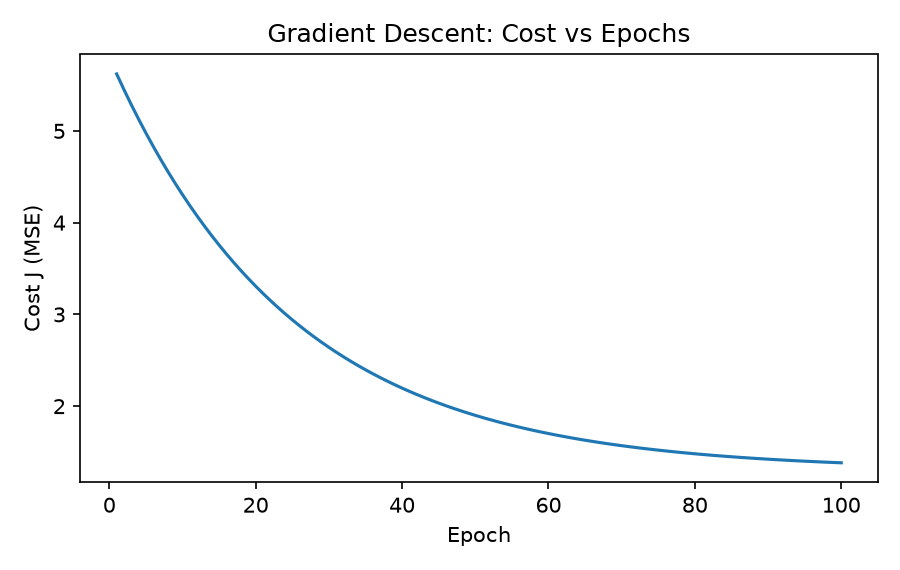
\includegraphics[width=0.62\textwidth]{exp4b_cost.png}\par
\small Fig. 2: Gradient-descent cost vs epochs ($\alpha=0.01$, 100 epochs).\par
\end{center}
\vspace{4pt}

\tooddpage
\expheading{RESULT}
\vspace{4pt}
{\fontsize{12}{15}\selectfont
The above program was implemented and executed successfully using Python, and the corresponding output was obtained and verified. The results of the \textbf{gradient descent regression} were analyzed and found to be satisfactory, thereby achieving the desired objective of the experiment.\par
}

\vspace{12pt}

\noindent\textbf{Faculty Signature:} \underline{\hspace{3.6cm}} \hfill \textbf{Date:} \underline{\hspace{2.8cm}}\par

\tooddpage

% ============================================================
% EXPERIMENT 4C
% ============================================================
{\setlength{\parskip}{1pt}\setlength{\abovedisplayskip}{2pt}\setlength{\belowdisplayskip}{2pt}
\begin{center}
\expheading{EXPERIMENT NO. 4C}
\end{center}
\vspace{2pt}

\noindent\textbf{Date:} 14-8-2026\par
\vspace{6pt}

\expheading{TITLE}
\vspace{4pt}
\noindent Simple Linear Regression with Scikit-learn -- AveRooms\par
\vspace{4pt}

\expheading{AIM}
\vspace{4pt}
\noindent To fit the sklearn LinearRegression model on AveRooms, predict test values, and assess with MSE and $R^2$. \par
\vspace{4pt}

\expheading{OBJECTIVE}
\vspace{2pt}
\fullrule
\vspace{4pt}
\noindent To implement simple linear regression with Scikit-learn on the California Housing dataset (X=AveRooms, Y=MedHouseVal) and evaluate it with MSE, R-squared and the regression-line plot. \par
\vspace{4pt}

\expheading{THEORY}
\vspace{4pt}
Linear hypothesis:
\[\hat{Y}=mX+b\]
Scikit-learn fits $m,b$ by least squares (normal equation via SVD).
Goodness of fit:
\[\mathrm{MSE}=\frac{1}{n}\sum_{i=1}^{n}(Y_i-\hat{Y}_i)^2\qquad R^2=1-\frac{\sum_{i=1}^{n}(Y_i-\hat{Y}_i)^2}{\sum_{i=1}^{n}(Y_i-\bar{Y})^2}\]
\vspace{4pt}

\expheading{PROCEDURE}
\vspace{4pt}
\noindent 1. Import NumPy and Pandas for data handling; fetch\_california\_housing, train\_test\_split, LinearRegression, mean\_squared\_error, r2\_score and Matplotlib.\par
\noindent 2. Load with fetch\_california\_housing(); build the DataFrame; assign feature names; separate the target.\par
\noindent 3. Explore: first records, shape, features and missing values.\par
\noindent 4. Take X=AveRooms, Y=MedHouseVal; scatter AveRooms vs MedHouseVal.\par
\noindent 5. Split 80/20 (random\_state=42); fit LinearRegression; read slope $m$ and intercept $b$.\par
\noindent 6. Predict test values; report MSE and $R^2$; plot test points with the regression line, labels, title and legend. \par
\vspace{4pt}

\expheading{DATASET DESCRIPTION}
\vspace{4pt}
\noindent Dataset Name: California Housing via Scikit-learn\par
\noindent Source: fetch\_california\_housing (1990 census)\par
\noindent Number of Samples: 20640 \hspace{0.3cm} Number of Features: 8 (X=AveRooms)\par
\noindent Target / Class: MedHouseVal $-$ median house value in units of \$100{,}000\par
\noindent Description: Train 16512 / test 4128 (80/20, random\_state=42). \par
\vspace{4pt}
} % end sheet-local tightening
\toevenpage
\expheading{PROGRAM}
\vspace{6pt}

\begin{lstlisting}
import numpy as np
import pandas as pd
import matplotlib
matplotlib.use("Agg")
import matplotlib.pyplot as plt
from sklearn.datasets import fetch_california_housing
from sklearn.model_selection import train_test_split
from sklearn.linear_model import LinearRegression
from sklearn.metrics import mean_squared_error, r2_score
housing = fetch_california_housing()
df = pd.DataFrame(housing.data, columns=housing.feature_names)
print("Shape:", df.shape)
print("Missing:", int(df.isnull().sum().sum()))
X = df[["AveRooms"]]
y = housing.target
X_train, X_test, y_train, y_test = train_test_split(
    X, y, test_size=0.2, random_state=42)
print("Train:", len(X_train), " Test:", len(X_test))
model = LinearRegression()
model.fit(X_train, y_train)
print(f"m = {model.coef_[0]:.6f} b = {model.intercept_:.4f}")
p = model.predict(X_test)
print(f"MSE={mean_squared_error(y_test, p):.4f} "
      f"R2={r2_score(y_test, p):.4f} RMSE={np.sqrt(mean_squared_error(y_test, p)):.4f}")
plt.figure(figsize=(7, 4.5))
plt.scatter(X_test, y_test, s=6, alpha=0.25, label="Test data")
xs = np.linspace(0, 15, 200)
plt.plot(xs, model.coef_[0] * xs + model.intercept_,
         linewidth=2, label="Sklearn line")
plt.xlim(0, 15)
plt.xlabel("AveRooms")
plt.ylabel("MedHouseVal ($100k)")
plt.title("Simple Linear Regression with Scikit-learn")
plt.legend()
plt.tight_layout()
plt.savefig("exp4c_fit.png", dpi=150)
\end{lstlisting}
\toevenpage
\expheading{OUTPUT}
\vspace{2pt}
\noindent\rule{\textwidth}{0.5pt}\par
\vspace{4pt}
\begin{verbatim}
Shape: (20640, 8)
Missing: 0
Train: 16512  Test: 4128
m = 0.076756 b = 1.6548
MSE=1.2923 R2=0.0138 RMSE=1.1368
\end{verbatim}
\vspace{4pt}

\begin{center}
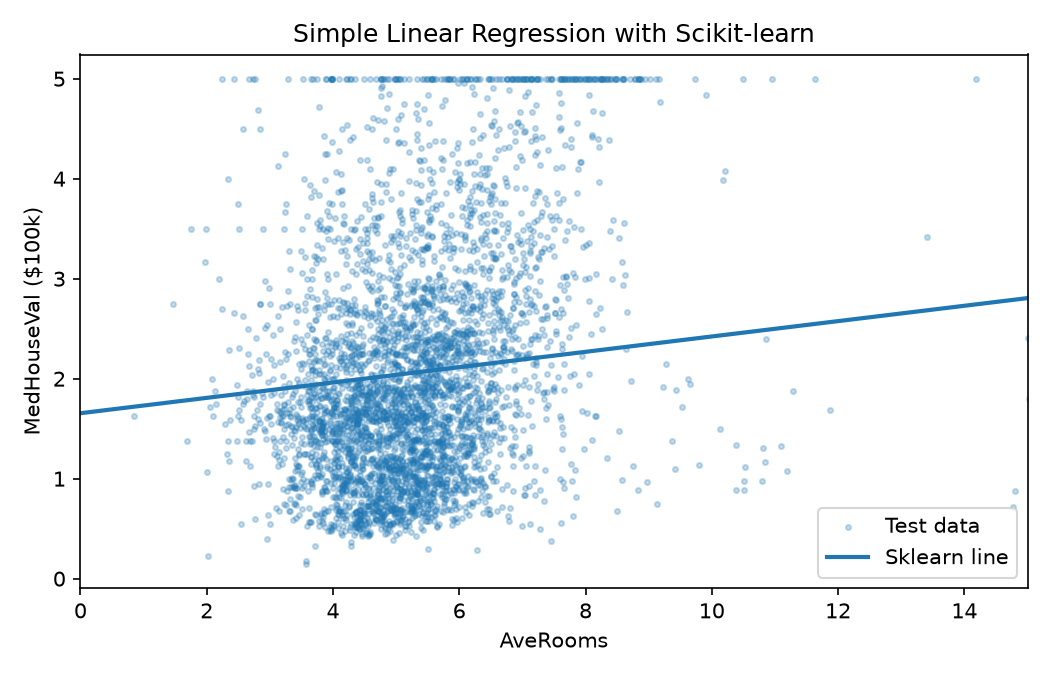
\includegraphics[width=0.78\textwidth]{exp4c_fit.png}\par
\small Fig. 1: Test data with the Scikit-learn regression line.\par
\end{center}
\vspace{4pt}

\tooddpage
\expheading{RESULT}
\vspace{4pt}
{\fontsize{12}{15}\selectfont
The above program was implemented and executed successfully using Python, and the corresponding output was obtained and verified. The results of the \textbf{Scikit-learn LinearRegression model} were analyzed and found to be satisfactory, thereby achieving the desired objective of the experiment.\par
}

\vspace{12pt}

\noindent\textbf{Faculty Signature:} \underline{\hspace{3.6cm}} \hfill \textbf{Date:} \underline{\hspace{2.8cm}}\par

\tooddpage

% ============================================================
% EXPERIMENT 5
% ============================================================
{\setlength{\parskip}{1pt}\setlength{\abovedisplayskip}{2pt}\setlength{\belowdisplayskip}{2pt}
\begin{center}
\expheading{EXPERIMENT NO. 5}
\end{center}
\vspace{2pt}

\noindent\textbf{Date:} 9-9-2026\par
\vspace{6pt}

\expheading{TITLE}
\vspace{4pt}
\noindent K-Nearest Neighbors Classification on Breast Cancer Dataset\par
\vspace{4pt}

\expheading{AIM}
\vspace{4pt}
\noindent To classify tumors with K-Nearest Neighbors for $K=3,5,7,9$ and compare precision, recall, F1-score and accuracy. \par
\vspace{4pt}

\expheading{OBJECTIVE}
\vspace{2pt}
\fullrule
\vspace{4pt}
\noindent To implement K-Nearest Neighbors for binary classification on the Breast Cancer dataset, evaluate K=3,5,7,9 with a comparison table and confusion matrix, and plot accuracy versus K. \par
\vspace{4pt}

\expheading{THEORY}
\vspace{4pt}
Majority vote of the $K$ neighbours:
\[\hat{y}=\arg\max_c\sum_{i\in N_K(x)}[y_i=c]\]
Euclidean distance:
\[d(x,z)=\sqrt{\sum_{j=1}^{30}(x_j-z_j)^2}\]
Binary metrics with TP, TN, FP, FN:
\[\text{Acc}=\frac{TP+TN}{TP+TN+FP+FN}\qquad \text{Prec}=\frac{TP}{TP+FP}\qquad \text{Rec}=\frac{TP}{TP+FN}\qquad F_1=2\frac{\text{Prec}\cdot\text{Rec}}{\text{Prec}+\text{Rec}}\]
\vspace{4pt}

\expheading{PROCEDURE}
\vspace{4pt}
\noindent 1. Import NumPy, Pandas, Matplotlib and sklearn (datasets, model\_selection, neighbors, metrics).\par
\noindent 2. Load the Breast Cancer dataset with load\_breast\_cancer(); separate 30 features $X$ and binary target $Y$.\par
\noindent 3. Split 80/20 (random\_state=42).\par
\noindent 4. Create KNeighborsClassifier with Euclidean distance ($p=2$), starting $K=3$.\par
\noindent 5. Train the model; predict the test samples.\par
\noindent 6. Compute accuracy, precision, recall, F1-score and confusion matrix.\par
\noindent 7. Repeat for $K=3,5,7,9$; display the comparison table.\par
\noindent 8. Plot accuracy versus $K$ ($K$ on X-axis, accuracy on Y-axis). \par
\vspace{4pt}

\expheading{DATASET DESCRIPTION}
\vspace{4pt}
\noindent Dataset Name: Breast Cancer Wisconsin (load\_breast\_cancer)\par
\noindent Source: 569 samples; 30 numerical features\par
\noindent Number of Samples: 455 train / 114 test \hspace{0.3cm} Number of Features: 30\par
\noindent Target / Class: binary (malignant/benign)\par
\noindent Description: 80/20 split, random\_state=42; Euclidean distance. \par
\vspace{4pt}
} % end sheet-local tightening
\toevenpage
\expheading{PROGRAM}
\vspace{6pt}

\begin{lstlisting}
import numpy as np
import pandas as pd
import matplotlib
matplotlib.use("Agg")
import matplotlib.pyplot as plt
from sklearn.datasets import load_breast_cancer
from sklearn.model_selection import train_test_split
from sklearn.neighbors import KNeighborsClassifier
from sklearn.metrics import accuracy_score, precision_score, recall_score, f1_score, confusion_matrix
data = load_breast_cancer()
X = pd.DataFrame(data.data, columns=data.feature_names)
y = pd.Series(data.target)
print("Samples:", X.shape, "Classes:", data.target_names.tolist())
X_train, X_test, y_train, y_test = train_test_split(X, y, test_size=0.2, random_state=42)
print("Train:", len(X_train), " Test:", len(X_test))
print("K  acc prec rec f1")
cm_best, best_a, best_k, acc = None, -1.0, 0, []
for K in [3, 5, 7, 9]:
    model = KNeighborsClassifier(n_neighbors=K, p=2)
    model.fit(X_train, y_train)
    p = model.predict(X_test)
    a = accuracy_score(y_test, p)
    acc.append(a)
    print(f"{K}  {a:.4f} {precision_score(y_test, p):.4f} {recall_score(y_test, p):.4f} {f1_score(y_test, p):.4f}")
    if a > best_a:
        best_a, best_k = a, K
        cm_best = confusion_matrix(y_test, p)
print("Confusion matrix at best K:")
print(cm_best)
print(f"Best K = {best_k}")
plt.figure(figsize=(7, 4.5))
plt.plot([3, 5, 7, 9], acc, marker="o", linewidth=2)
plt.xlabel("K")
plt.ylabel("Test accuracy")
plt.title("KNN on Breast Cancer: Accuracy vs K")
plt.grid(True)
plt.tight_layout()
plt.savefig("exp5_knn_acc.png", dpi=150)
\end{lstlisting}
\toevenpage
\expheading{OUTPUT}
\vspace{2pt}
\noindent\rule{\textwidth}{0.5pt}\par
\vspace{4pt}
\begin{verbatim}
Samples: (569, 30) Classes: ['malignant', 'benign']
Train: 455  Test: 114
K  acc prec rec f1
3  0.9298 0.9315 0.9577 0.9444
5  0.9561 0.9342 1.0000 0.9660
7  0.9561 0.9459 0.9859 0.9655
9  0.9561 0.9459 0.9859 0.9655
Confusion matrix at best K:
[[38  5]
 [ 0 71]]
Best K = 5
\end{verbatim}
\vspace{4pt}

\begin{center}
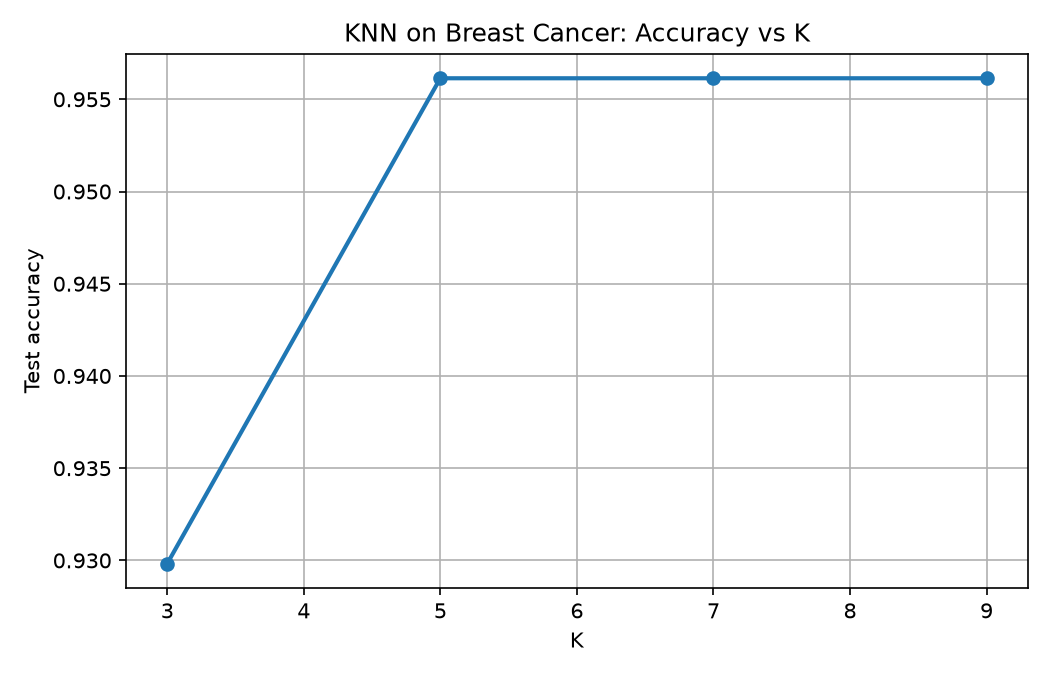
\includegraphics[width=0.78\textwidth]{exp5_knn_acc.png}\par
\small Fig. 1: Test accuracy vs $K$ (best $K=5$).\par
\end{center}
\vspace{4pt}

\tooddpage
\expheading{RESULT}
\vspace{4pt}
{\fontsize{12}{15}\selectfont
The above program was implemented and executed successfully using Python, and the corresponding output was obtained and verified. The results of the \textbf{K-Nearest Neighbors classifier} were analyzed and found to be satisfactory, thereby achieving the desired objective of the experiment.\par
}

\vspace{12pt}

\noindent\textbf{Faculty Signature:} \underline{\hspace{3.6cm}} \hfill \textbf{Date:} \underline{\hspace{2.8cm}}\par

\tooddpage

% ============================================================
% EXPERIMENT 6
% ============================================================
{\setlength{\parskip}{1pt}\setlength{\abovedisplayskip}{2pt}\setlength{\belowdisplayskip}{2pt}
\begin{center}
\expheading{EXPERIMENT NO. 6}
\end{center}
\vspace{2pt}

\noindent\textbf{Date:} 9-9-2026\par
\vspace{6pt}

\expheading{TITLE}
\vspace{4pt}
\noindent Customer Segmentation using Decision Tree\par
\vspace{4pt}

\expheading{AIM}
\vspace{4pt}
\noindent Customer Segmentation using a Decision Tree classifier on the Online Retail Dataset. \par
\vspace{4pt}

\expheading{OBJECTIVE}
\vspace{2pt}
\fullrule
\vspace{4pt}
\noindent To segment customers with a Decision Tree classifier (entropy criterion) on Online Retail data, visualize the tree, analyze feature importance, and discuss how the structure explains purchasing behavior. \par
\vspace{4pt}

\expheading{THEORY}
\vspace{4pt}
Entropy of a node:
\[H(S)=-\sum_c p_c\log_2 p_c\]
Information gain of a split:
\[G(S,f)=H(S)-\sum_v\frac{|S_v|}{|S|}H(S_v)\]
The tree splits on $x_j \le t$ with maximum gain (max depth 3); feature importance is the normalized total gain decrease.
\vspace{4pt}

\expheading{PROCEDURE}
\vspace{4pt}
\noindent 1. Load the Online Retail dataset (UCI).\par
\noindent 2. Clean data (drop missing CustomerID; keep Quantity$>0$, UnitPrice$>0$).\par
\noindent 3. Create per-customer features (Recency, Frequency, Monetary, AvgBasket, Items).\par
\noindent 4. Define target (Monetary terciles); 80/20 split (random\_state=42).\par
\noindent 5. Fit DecisionTreeClassifier (entropy, max depth 3).\par
\noindent 6. Visualize the tree with plot\_tree.\par
\noindent 7. Analyze feature importance. \par
\vspace{4pt}

\expheading{DATASET DESCRIPTION}
\vspace{4pt}
\noindent Dataset Name: Online Retail (UCI, online\_retail.zip)\par
\noindent Source: 541909 rows $\rightarrow$ 397884 clean $\rightarrow$ 4338 customers\par
\noindent Number of Samples: 3470 train / 868 test \hspace{0.3cm} Number of Features: 4\par
\noindent Target / Class: value segment (0/1/2)\par
\noindent Description: seed 42 via random\_state; depth 3. \par
\vspace{4pt}
} % end sheet-local tightening
\toevenpage
\expheading{PROGRAM}
\vspace{6pt}

\begin{lstlisting}
import os
import urllib.request
import zipfile
import numpy as np
import pandas as pd
import matplotlib
matplotlib.use("Agg")
import matplotlib.pyplot as plt
from sklearn.model_selection import train_test_split
from sklearn.tree import DecisionTreeClassifier, plot_tree
from sklearn.metrics import accuracy_score
ZP = "online_retail.zip"
if not os.path.exists(ZP):
    print("Downloading Online Retail")
    urllib.request.urlretrieve("https://archive.ics.uci.edu/static/public/352/online+retail.zip", ZP)
with zipfile.ZipFile(ZP) as z:
    name = [n for n in z.namelist() if n.endswith(".xlsx")][0]
    df = pd.read_excel(z.open(name), engine="openpyxl")
print("Rows:", len(df))
df = df.dropna(subset=["CustomerID"])
df = df[(df["Quantity"] > 0) & (df["UnitPrice"] > 0)]
print("Clean rows:", len(df))
df["Total"] = df["Quantity"] * df["UnitPrice"]
maxd = df["InvoiceDate"].max()
g = df.groupby("CustomerID")
cust = pd.DataFrame({
    "Recency": (maxd - g["InvoiceDate"].max()).dt.days,
    "Frequency": g["InvoiceNo"].nunique(),
    "Monetary": g["Total"].sum(),
    "AvgBasket": g["Total"].mean(),
    "Items": g["StockCode"].nunique(),
})
print("Customers:", len(cust))
m = cust["Monetary"].values
y = np.where(m <= np.percentile(m, 33.3), 0, np.where(m <= np.percentile(m, 66.7), 1, 2))
X = cust[["Recency", "Frequency", "AvgBasket", "Items"]]
print("Classes:", np.bincount(y).tolist())
X_train, X_test, y_train, y_test = train_test_split(X, y, test_size=0.2, random_state=42)
print("Train:", len(X_train), " Test:", len(X_test))
\end{lstlisting}

\toevenpage
\expheading{PROGRAM (continued)}
\vspace{6pt}

\begin{lstlisting}
model = DecisionTreeClassifier(criterion="entropy", max_depth=3, random_state=42)
model.fit(X_train, y_train)
p = model.predict(X_test)
print(f"DecisionTree: acc={accuracy_score(y_test, p):.4f} depth={model.get_depth()} leaves={model.get_n_leaves()}")
print("Importance:", " ".join(f"{f}={v:.3f}" for f, v in zip(X.columns, model.feature_importances_)))
plt.figure(figsize=(12, 7))
plot_tree(model, feature_names=list(X.columns), class_names=["Low", "Mid", "High"], filled=True, rounded=True, fontsize=8)
plt.title("Decision Tree (entropy) for Customer Segments")
plt.tight_layout()
plt.savefig("exp6_tree.png", dpi=150)
plt.figure(figsize=(7, 4))
plt.barh(list(X.columns), model.feature_importances_)
plt.xlabel("Importance")
plt.title("Decision Tree Feature Importance")
plt.tight_layout()
plt.savefig("exp6_imp.png", dpi=150)
\end{lstlisting}
\toevenpage
\expheading{OUTPUT}
\vspace{2pt}
\noindent\rule{\textwidth}{0.5pt}\par
\vspace{4pt}
\begin{verbatim}
Rows: 541909
Clean rows: 397884
Customers: 4338
Classes: [1445, 1448, 1445]
Train: 3470  Test: 868
DecisionTree: acc=0.7131 depth=3 leaves=8
Importance: Recency=0.000 Frequency=0.584 AvgBasket=0.213 Items=0.203
\end{verbatim}
\vspace{4pt}

\begin{center}
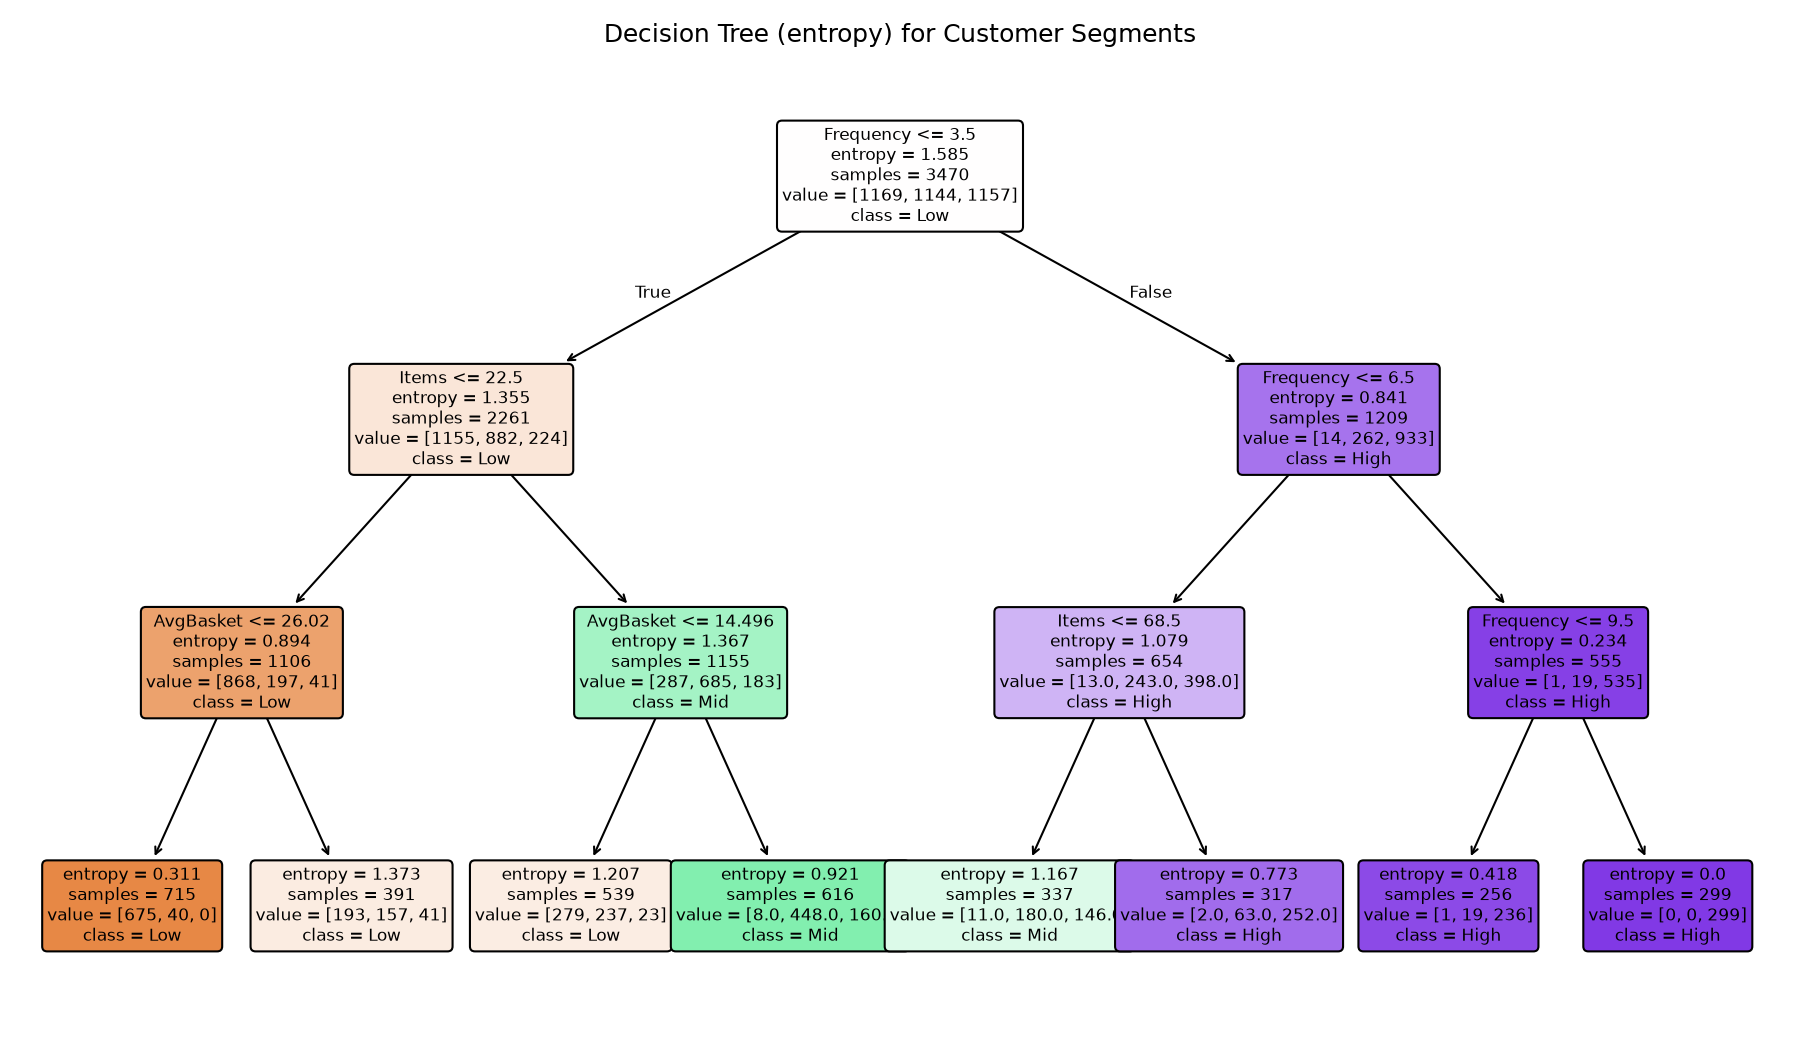
\includegraphics[width=0.90\textwidth]{exp6_tree.png}\par
\small Fig. 1: Decision tree (Frequency root, depth 3).\par
\vspace{6pt}
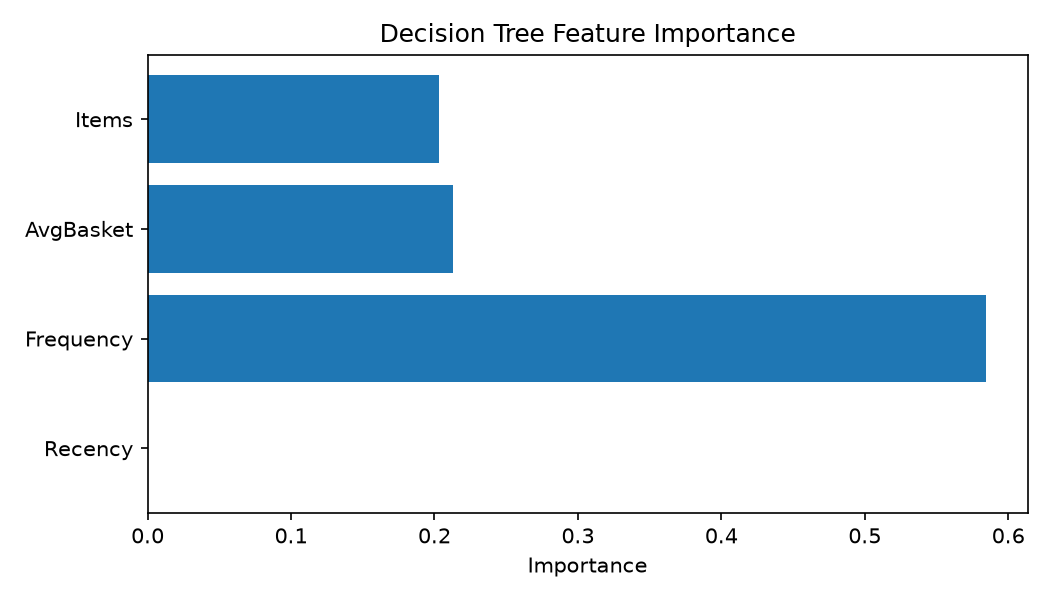
\includegraphics[width=0.62\textwidth]{exp6_imp.png}\par
\small Fig. 2: Feature importance (Frequency leads).\par
\end{center}
\vspace{4pt}

\tooddpage
\expheading{RESULT}
\vspace{4pt}
{\fontsize{12}{15}\selectfont
The above program was implemented and executed successfully using Python, and the corresponding output was obtained and verified. The results of the \textbf{Decision Tree classifier} were analyzed and found to be satisfactory, thereby achieving the desired objective of the experiment.\par
}

\vspace{12pt}

\noindent\textbf{Faculty Signature:} \underline{\hspace{3.6cm}} \hfill \textbf{Date:} \underline{\hspace{2.8cm}}\par

\tooddpage

% ============================================================
% EXPERIMENT 7
% ============================================================
{\setlength{\parskip}{1pt}\setlength{\abovedisplayskip}{2pt}\setlength{\belowdisplayskip}{2pt}
\begin{center}
\expheading{EXPERIMENT NO. 7}
\end{center}
\vspace{2pt}

\noindent\textbf{Date:} 07-10-2026\par
\vspace{6pt}

\expheading{TITLE}
\vspace{4pt}
\noindent Logistic Regression with and without Feature Scaling on Pima Indian Diabetes Dataset\par
\vspace{4pt}

\expheading{AIM}
\vspace{4pt}
\noindent To implement a Logistic Regression model to predict the likelihood of disease using the Pima Indian Diabetes dataset and compare its performance with and without feature scaling. \par
\vspace{4pt}

\expheading{OBJECTIVE}
\vspace{2pt}
\fullrule
\vspace{4pt}
\noindent To implement Logistic Regression on the Pima Indian Diabetes dataset, evaluate its performance using classification metrics, and study the effect of feature scaling on the model performance. \par
\vspace{4pt}

\expheading{THEORY}
\vspace{4pt}
Logistic Regression is a supervised machine learning algorithm used for binary classification. It predicts the probability of a sample belonging to a particular class using the sigmoid function:
\[P(Y=1|X)=\frac{1}{1+e^{-z}}\]
where
\[z=\beta_0+\beta_1X_1+\beta_2X_2+\cdots+\beta_nX_n\]
The predicted probability is converted into a class label using a classification threshold. Feature scaling transforms the input features to a common scale using standardization:
\[z=\frac{x-\mu}{\sigma}\]
where $\mu$ is the mean of the feature and $\sigma$ is its standard deviation.
\vspace{4pt}

\expheading{PROCEDURE}
\vspace{4pt}
\noindent 1. Load dataset and generate description\par
\noindent 2. Split into training and testing sets\par
\noindent 3. Train model without scaling\par
\noindent 4. Evaluate performance\par
\noindent 5. Apply feature scaling\par
\noindent 6. Train again\par
\noindent 7. Compare results \par
\vspace{4pt}

\expheading{DATASET DESCRIPTION}
\vspace{4pt}
\noindent Dataset Name: Pima Indian Diabetes Dataset\par
\noindent Source: diabetes.csv\par
\noindent Number of Samples: 768 \hspace{0.3cm} Number of Features: 8\par
\noindent Features: Pregnancies, Glucose, BloodPressure, SkinThickness, Insulin, BMI, DiabetesPedigreeFunction, Age\par
\noindent Target / Class: Outcome \par
\vspace{4pt}
} % end sheet-local tightening
\toevenpage
\expheading{PROGRAM}
\vspace{6pt}

\begin{lstlisting}
import pandas as pd
from sklearn.model_selection import train_test_split
from sklearn.preprocessing import StandardScaler
from sklearn.linear_model import LogisticRegression
from sklearn.metrics import accuracy_score, precision_score, recall_score, f1_score
df = pd.read_csv("diabetes.csv")
print("Dataset:", df.shape)
data = df.drop(columns=["Outcome"])
y = df["Outcome"]
X_train, X_test, y_train, y_test = train_test_split(data, y, test_size=0.2, random_state=42)
print("Train:", len(X_train), " Test:", len(X_test))
model = LogisticRegression(max_iter=1000)
model.fit(X_train, y_train)
p = model.predict(X_test)
print("Without scaling:")
print(f"acc={accuracy_score(y_test, p):.4f} prec={precision_score(y_test, p):.4f} rec={recall_score(y_test, p):.4f} f1={f1_score(y_test, p):.4f}")
scaler = StandardScaler()
X_train_s = scaler.fit_transform(X_train)
X_test_s = scaler.transform(X_test)
model_s = LogisticRegression(max_iter=1000)
model_s.fit(X_train_s, y_train)
ps = model_s.predict(X_test_s)
print("With scaling:")
print(f"acc={accuracy_score(y_test, ps):.4f} prec={precision_score(y_test, ps):.4f} rec={recall_score(y_test, ps):.4f} f1={f1_score(y_test, ps):.4f}")
diff = accuracy_score(y_test, ps) - accuracy_score(y_test, p)
print(f"Accuracy changed by {diff:+.4f} after scaling")
\end{lstlisting}
\toevenpage
\expheading{OUTPUT}
\vspace{2pt}
\noindent\rule{\textwidth}{0.5pt}\par
\vspace{4pt}
\begin{verbatim}
Dataset: (768, 9)
Train: 614  Test: 154
Without scaling:
acc=0.7468 prec=0.6379 rec=0.6727 f1=0.6549
With scaling:
acc=0.7532 prec=0.6491 rec=0.6727 f1=0.6607
Accuracy changed by +0.0065 after scaling
\end{verbatim}
\vspace{4pt}

\tooddpage
\expheading{RESULT}
\vspace{4pt}
{\fontsize{12}{15}\selectfont
The above program was implemented and executed successfully using Python, and the corresponding output was obtained and verified. The results of the \textbf{Logistic Regression model} were analyzed and found to be satisfactory, thereby achieving the desired objective of the experiment.\par
}

\vspace{12pt}

\noindent\textbf{Faculty Signature:} \underline{\hspace{3.6cm}} \hfill \textbf{Date:} \underline{\hspace{2.8cm}}\par

\tooddpage

% ============================================================
% EXPERIMENT 8
% ============================================================
{\setlength{\parskip}{1pt}\setlength{\abovedisplayskip}{2pt}\setlength{\belowdisplayskip}{2pt}
\begin{center}
\expheading{EXPERIMENT NO. 8}
\end{center}
\vspace{2pt}

\noindent\textbf{Date:} 07-10-2026\par
\vspace{6pt}

\expheading{TITLE}
\vspace{4pt}
\noindent Ridge and Lasso Regularization on Diabetes Dataset\par
\vspace{4pt}

\expheading{AIM}
\vspace{4pt}
\noindent To implement Ridge and Lasso regularization on the Diabetes dataset and compare the performance of these regularized models with standard Multiple Linear Regression. \par
\vspace{4pt}

\expheading{OBJECTIVE}
\vspace{2pt}
\fullrule
\vspace{4pt}
\noindent To compare Ordinary Least Squares (OLS), Ridge Regression, and Lasso Regression using Mean Squared Error (MSE) and R$^2$ score, and visualize their performance. \par
\vspace{4pt}

\expheading{THEORY}
\vspace{4pt}
Multiple Linear Regression is a supervised learning algorithm used to predict a continuous target variable using multiple input features. The model is given by:
\[\hat{y}=\beta_0+\beta_1X_1+\beta_2X_2+\cdots+\beta_nX_n\]
Ordinary Least Squares (OLS) estimates the coefficients by minimizing the sum of squared errors. Ridge and Lasso Regression are regularized forms of linear regression that add penalty terms to reduce overfitting.
\[J(\beta)=\frac{1}{n}\sum_{i=1}^{n}(y_i-\hat{y}_i)^2+\lambda\sum_{j=1}^{n}\beta_j^2\]
Ridge (L2) reduces the magnitude of the coefficients while retaining all the features.
\[J(\beta)=\frac{1}{n}\sum_{i=1}^{n}(y_i-\hat{y}_i)^2+\lambda\sum_{j=1}^{n}\lvert\beta_j\rvert\]
Lasso (L1) can reduce some coefficients exactly to zero and therefore performs feature selection.
\vspace{4pt}

\expheading{PROCEDURE}
\vspace{4pt}
\noindent 1. Load the dataset and generate description\par
\noindent 2. Split into train and test sets\par
\noindent 3. Train:\par
\noindent\hspace*{0.55cm}$\circ$~Linear Regression\par
\noindent\hspace*{0.55cm}$\circ$~Ridge Regression\par
\noindent\hspace*{0.55cm}$\circ$~Lasso Regression\par
\noindent 4. Evaluate using MSE and R$^2$\par
\noindent 5. Plot regression curves\par
\noindent 6. Compare coefficients \par
\vspace{4pt}

\expheading{DATASET DESCRIPTION}
\vspace{4pt}
\noindent Dataset Name: Diabetes Dataset\par
\noindent Source: Scikit-learn\par
\noindent Number of Samples: 442 (353 train / 89 test) \hspace{0.3cm} Number of Features: 10\par
\noindent Features: Age, Sex, BMI, BP, S1, S2, S3, S4, S5 and S6\par
\noindent Target: Disease progression \par
\vspace{4pt}
} % end sheet-local tightening
\toevenpage
\expheading{PROGRAM}
\vspace{6pt}

\begin{lstlisting}
import numpy as np
import matplotlib
matplotlib.use("Agg")
import matplotlib.pyplot as plt
from sklearn.datasets import load_diabetes
from sklearn.model_selection import train_test_split
from sklearn.linear_model import LinearRegression, Ridge, Lasso
from sklearn.metrics import mean_squared_error, r2_score
data = load_diabetes()
X = data.data
y = data.target
print("Samples:", X.shape)
print("Features:", " ".join(data.feature_names))
X_train, X_test, y_train, y_test = train_test_split(X, y, test_size=0.2, random_state=42)
print("Train:", len(X_train), " Test:", len(X_test))
models = [("Linear", LinearRegression()), ("Ridge", Ridge(alpha=1.0)), ("Lasso", Lasso(alpha=1.0))]
print("Model             MSE       R2")
for name, m in models:
    m.fit(X_train, y_train)
    p = m.predict(X_test)
    mse = mean_squared_error(y_test, p)
    r2 = r2_score(y_test, p)
    print(f"{name:14s} {mse:9.2f} {r2:9.4f}")
    if name == "Linear":
        py = p
    if name == "Ridge":
        pr = p
    if name == "Lasso":
        pl = p
\end{lstlisting}

\toevenpage
\expheading{PROGRAM (continued)}
\vspace{6pt}

\begin{lstlisting}
plt.figure(figsize=(6.5, 4.5))
plt.scatter(y_test, py, s=18, label="Linear")
plt.scatter(y_test, pr, s=18, label="Ridge")
plt.scatter(y_test, pl, s=18, label="Lasso")
lo, hi = y_test.min(), y_test.max()
plt.plot([lo, hi], [lo, hi], "k--")
plt.xlabel("Actual")
plt.ylabel("Predicted")
plt.title("Diabetes: Actual vs Predicted")
plt.legend()
plt.grid(True)
plt.tight_layout()
plt.savefig("exp8_pred.png", dpi=150)
pos = np.arange(len(data.feature_names))
plt.figure(figsize=(7, 4.5))
for (name, m), off in zip(models, [-0.26, 0.0, 0.26]):
    plt.barh(pos + off, m.coef_, height=0.26, label=name)
plt.yticks(pos, data.feature_names)
plt.axvline(0, color="k", linewidth=0.8)
plt.xlabel("Coefficient")
plt.title("Coefficient Comparison")
plt.legend()
plt.tight_layout()
plt.savefig("exp8_coef.png", dpi=150)
print("Lasso zeroed", int(np.sum(models[2][1].coef_ == 0)), "of 10 coefficients")
\end{lstlisting}
\toevenpage
\expheading{OUTPUT}
\vspace{2pt}
\noindent\rule{\textwidth}{0.5pt}\par
\vspace{4pt}
\begin{verbatim}
Samples: (442, 10)
Features: age sex bmi bp s1 s2 s3 s4 s5 s6
Train: 353  Test: 89
Model             MSE       R2
Linear           2900.19    0.4526
Ridge            3077.42    0.4192
Lasso            3403.58    0.3576
Lasso zeroed 7 of 10 coefficients
\end{verbatim}
\vspace{4pt}

\begin{center}
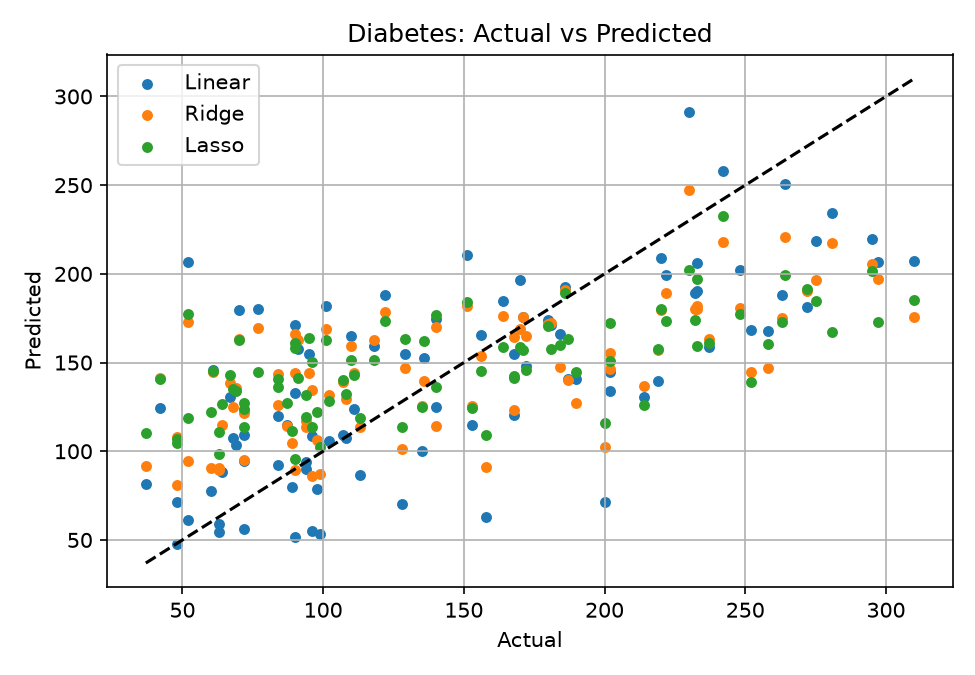
\includegraphics[width=0.70\textwidth]{exp8_pred.png}\par
\small Fig. 1: Actual vs predicted on the test set.\par
\vspace{6pt}
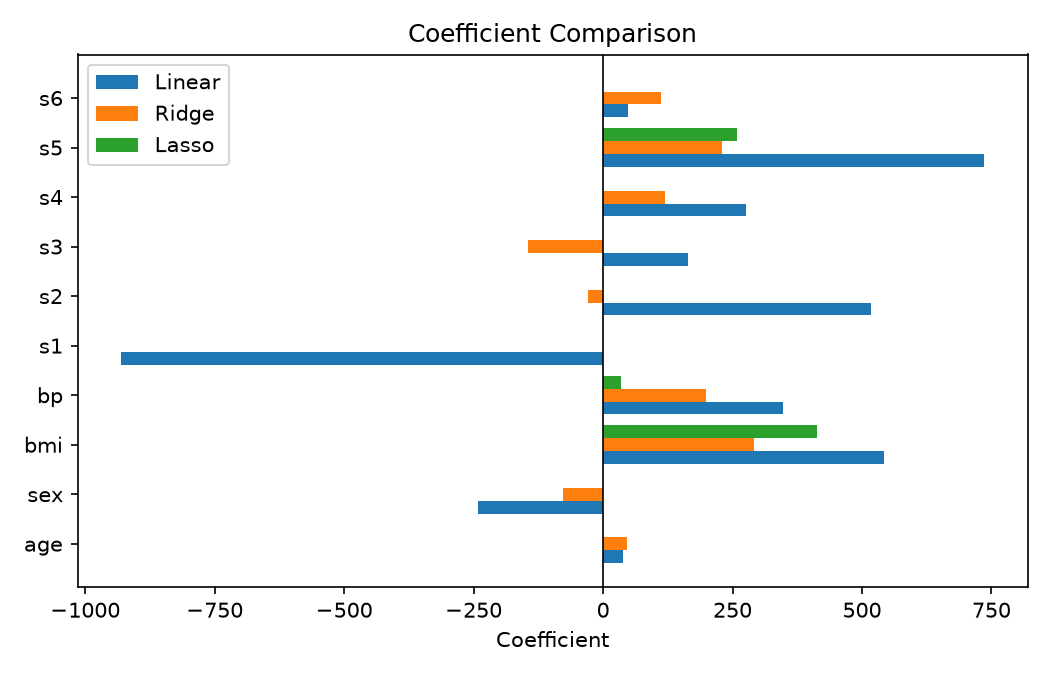
\includegraphics[width=0.74\textwidth]{exp8_coef.png}\par
\small Fig. 2: Coefficient comparison (Lasso zeroed 7 coefficients).\par
\end{center}
\vspace{4pt}

\tooddpage
\expheading{RESULT}
\vspace{4pt}
{\fontsize{12}{15}\selectfont
The above program was implemented and executed successfully using Python, and the corresponding output was obtained and verified. The results of the \textbf{Ridge and Lasso Regression} were analyzed and found to be satisfactory, thereby achieving the desired objective of the experiment.\par
}

\vspace{12pt}

\noindent\textbf{Faculty Signature:} \underline{\hspace{3.6cm}} \hfill \textbf{Date:} \underline{\hspace{2.8cm}}\par

\tooddpage

% ============================================================
% EXPERIMENT 9
% ============================================================
{\makeatletter\let\vspace\@gobble\makeatother\setlength{\parskip}{0pt}\setlength{\abovedisplayskip}{0pt}\setlength{\belowdisplayskip}{0pt}
\begin{center}
\expheading{EXPERIMENT NO. 9}
\end{center}
\vspace{2pt}

\noindent\textbf{Date:} 14-10-2026\par
\vspace{6pt}

\expheading{TITLE}
\vspace{4pt}
\noindent Logistic Regression using MLE and MAP on Breast Cancer Wisconsin Dataset\par
\vspace{4pt}

\expheading{AIM}
\vspace{4pt}
\noindent To estimate the parameters of Logistic Regression using Maximum Likelihood Estimation (MLE) and Maximum A Posteriori (MAP) estimation on the Breast Cancer Wisconsin dataset and compare their performance. \par
\vspace{4pt}

\expheading{OBJECTIVE}
\vspace{2pt}
\fullrule
\vspace{4pt}
\noindent To implement Logistic Regression using MLE without regularization, MAP with L2 regularization, and MAP with L1 regularization, and compare their performance using classification metrics. \par
\vspace{4pt}

\expheading{THEORY}
\vspace{4pt}
Logistic Regression is a supervised machine learning algorithm used for binary classification. It predicts the probability of a sample belonging to a particular class using the sigmoid function:
\[P(Y=1|X)=\frac{1}{1+e^{-(\beta_0+\beta_1X_1+\beta_2X_2+\cdots+\beta_nX_n)}}\]
Maximum Likelihood Estimation (MLE) estimates the model parameters by maximizing the likelihood of observing the given training data; it uses no regularization penalty. Maximum A Posteriori (MAP) estimation incorporates prior information about the parameters along with the likelihood. Regularization can be used to perform MAP estimation.
\[J(\beta)=J_{\text{MLE}}+\lambda\sum_{j=1}^{n}\beta_j^2\]
L2 regularization reduces the magnitude of the coefficients and helps prevent overfitting.
\[J(\beta)=J_{\text{MLE}}+\lambda\sum_{j=1}^{n}\lvert\beta_j\rvert\]
L1 regularization can reduce some coefficients to zero and can therefore perform feature selection.
\vspace{4pt}

\expheading{PROCEDURE}
\vspace{4pt}
\noindent Load the dataset and separate the input features $X$ and target variable $y$.\par
\noindent Preprocess the data by handling missing values and splitting the data into training and testing sets.\par
\noindent Standardize the features using StandardScaler so that the variables are on a comparable scale.\par
\noindent Implement MLE Logistic Regression without regularization.\par
\noindent\hspace*{0.55cm}$\bullet$~Fit the model using the training data.\par
\noindent\hspace*{0.55cm}$\bullet$~Obtain the coefficient estimates and predictions.\par
\noindent Implement MAP Logistic Regression with L2 prior (Ridge).\par
\noindent\hspace*{0.55cm}$\bullet$~Apply L2 regularization using penalty='l2'.\par
\noindent\hspace*{0.55cm}$\bullet$~Train the model and obtain its coefficient estimates and predictions.\par
\noindent\hspace*{0.55cm}$\bullet$~L2 regularization shrinks coefficients toward zero.\par
\noindent Implement MAP Logistic Regression with L1 prior (Lasso).\par
\noindent\hspace*{0.55cm}$\bullet$~Apply L1 regularization using penalty='l1'.\par
\noindent\hspace*{0.55cm}$\bullet$~Train the model and obtain its coefficient estimates and predictions.\par
\noindent\hspace*{0.55cm}$\bullet$~L1 regularization can make some coefficients exactly zero.\par
\noindent Evaluate all three models using suitable metrics such as:\par
\noindent\hspace*{0.55cm}$\bullet$~Accuracy\par
\noindent\hspace*{0.55cm}$\bullet$~Precision\par
\noindent\hspace*{0.55cm}$\bullet$~Recall\par
\noindent\hspace*{0.55cm}$\bullet$~F1-score\par
\noindent Compare the parameter estimates (coefficients) obtained from MLE, MAP-L2, and MAP-L1 models. \par
\vspace{4pt}

\expheading{DATASET DESCRIPTION}
\vspace{4pt}
\noindent Dataset Name: Breast Cancer Wisconsin Dataset \hspace{0.3cm} Source: Scikit-learn\par
\noindent Number of Samples: 569 (455 train / 114 test) \hspace{0.3cm} Number of Features: 30\par
\noindent Features: Breast cancer diagnostic features \hspace{0.3cm} Target: Malignant / Benign \par
\vspace{4pt}
} % end sheet-local tightening
\toevenpage
\expheading{PROGRAM}
\vspace{6pt}

\begin{lstlisting}
import numpy as np
from sklearn.datasets import load_breast_cancer
from sklearn.model_selection import train_test_split
from sklearn.preprocessing import StandardScaler
from sklearn.linear_model import LogisticRegression
from sklearn.metrics import accuracy_score, precision_score, recall_score, f1_score
data = load_breast_cancer()
X = data.data
y = data.target
X_train, X_test, y_train, y_test = train_test_split(X, y, test_size=0.2, random_state=42, stratify=y)
print("Samples:", X.shape, "Train:", len(X_train), " Test:", len(X_test))
scaler = StandardScaler()
X_train_s = scaler.fit_transform(X_train)
X_test_s = scaler.transform(X_test)
models = [
    ("MLE", LogisticRegression(C=np.inf, max_iter=5000)),
    ("MAP L2", LogisticRegression(C=1.0, max_iter=5000)),
    ("MAP L1", LogisticRegression(l1_ratio=1, C=1.0, solver="saga", max_iter=5000)),
]
print("Model     acc    prec   rec    f1     nonzero")
for name, m in models:
    m.fit(X_train_s, y_train)
    p = m.predict(X_test_s)
    nz = int(np.sum(m.coef_[0] != 0))
    print(f"{name:8s} {accuracy_score(y_test, p):.4f} {precision_score(y_test, p):.4f} {recall_score(y_test, p):.4f} {f1_score(y_test, p):.4f} {nz}")
\end{lstlisting}
\toevenpage
\expheading{OUTPUT}
\vspace{2pt}
\noindent\rule{\textwidth}{0.5pt}\par
\vspace{4pt}
\begin{verbatim}
Samples: (569, 30) Train: 455  Test: 114
Model     acc    prec   rec    f1     nonzero
MLE      0.9211 0.9701 0.9028 0.9353 30
MAP L2   0.9825 0.9861 0.9861 0.9861 30
MAP L1   0.9912 0.9863 1.0000 0.9931 18
\end{verbatim}
\vspace{4pt}

\tooddpage
\expheading{RESULT}
\vspace{4pt}
{\fontsize{12}{15}\selectfont
The above program was implemented and executed successfully using Python, and the corresponding output was obtained and verified. The results of the \textbf{Logistic Regression with MLE and MAP estimation} were analyzed and found to be satisfactory, thereby achieving the desired objective of the experiment.\par
}

\vspace{12pt}

\noindent\textbf{Faculty Signature:} \underline{\hspace{3.6cm}} \hfill \textbf{Date:} \underline{\hspace{2.8cm}}\par

\tooddpage

% ============================================================
% EXPERIMENT 10
% ============================================================
{\makeatletter\let\vspace\@gobble\makeatother\setlength{\parskip}{0pt}\setlength{\abovedisplayskip}{0pt}\setlength{\belowdisplayskip}{0pt}
\begin{center}
\expheading{EXPERIMENT NO. 10}
\end{center}
\vspace{2pt}

\noindent\textbf{Date:} 14-10-2026\par
\vspace{6pt}

\expheading{TITLE}
\vspace{4pt}
\noindent K-Means Clustering on Digits Dataset\par
\vspace{4pt}

\expheading{AIM}
\vspace{4pt}
\noindent To implement the K-Means clustering algorithm on the Digits dataset and determine the optimal number of clusters using the elbow method and the silhouette score. \par
\vspace{4pt}

\expheading{OBJECTIVE}
\vspace{2pt}
\fullrule
\vspace{4pt}
\noindent To apply K-Means clustering with different values of K on the Digits dataset, evaluate the clustering using inertia and silhouette score, and identify the best K. \par
\vspace{4pt}

\expheading{THEORY}
\vspace{4pt}
K-Means is an unsupervised learning algorithm that partitions the data into K clusters. Each cluster is represented by its centroid, the mean of its member points:
\[\mu_c=\frac{1}{|C_c|}\sum_{x_i\in C_c}x_i\]
The algorithm alternates between assigning every point to its nearest centroid,
\[c(x)=\arg\min_c \lVert x-\mu_c\rVert^2\]
and recomputing the centroids, thereby minimizing the inertia (within-cluster sum of squares):
\[J=\sum_{c=1}^{K}\sum_{x\in C_c}\lVert x-\mu_c\rVert^2\]
The elbow method plots the inertia against K and looks for the point where the decrease flattens. The silhouette score measures how well each point fits its own cluster compared to the other clusters:
\[s(x)=\frac{b(x)-a(x)}{\max(a(x),\,b(x))}\]
where $a(x)$ is the mean distance to the points of its own cluster and $b(x)$ is the smallest mean distance to the points of any other cluster.
\vspace{4pt}

\expheading{PROCEDURE}
\vspace{4pt}
\noindent Load the Digits dataset using load\_digits() from sklearn.datasets.\par
\noindent Extract the features from the dataset. Each digit image is represented by 64 pixel features.\par
\noindent Preprocess the data by standardizing the features using StandardScaler.\par
\noindent Select different values of K, for example, K=2 to K=15.\par
\noindent Apply K-Means clustering for each selected value of K and assign every data point to a cluster.\par
\noindent Calculate the inertia for each K to measure the compactness of the clusters.\par
\noindent Calculate the silhouette score for each K to measure how well-separated the clusters are.\par
\noindent Plot the Elbow Curve using K and inertia to identify a suitable number of clusters.\par
\noindent Plot the Silhouette Score against K and identify the K value with a higher silhouette score. \par
\vspace{4pt}

\expheading{DATASET DESCRIPTION}
\vspace{4pt}
\noindent Dataset Name: Digits Dataset \hspace{0.3cm} Source: Scikit-learn (load\_digits)\par
\noindent Number of Samples: 1797 \hspace{0.3cm} Number of Features: 64\par
\noindent Classes: 10 digits (0--9)\par
\noindent Description: 8x8 grayscale digit images flattened to 64 features; standardized with StandardScaler before clustering. \par
\vspace{4pt}
} % end sheet-local tightening
\toevenpage
\expheading{PROGRAM}
\vspace{6pt}

\begin{lstlisting}
import numpy as np
import matplotlib
matplotlib.use("Agg")
import matplotlib.pyplot as plt
from sklearn.datasets import load_digits
from sklearn.preprocessing import StandardScaler
from sklearn.cluster import KMeans
from sklearn.metrics import silhouette_score
X, y = load_digits(return_X_y=True)
X = StandardScaler().fit_transform(X)
print("Digits:", X.shape)
print("Classes:", np.bincount(y).tolist())
Ks, inertias, silhouettes = [], [], []
for k in [2, 5, 8, 10, 12, 15]:
    km = KMeans(n_clusters=k, n_init=10, random_state=42)
    labels = km.fit_predict(X)
    sil = silhouette_score(X, labels)
    Ks.append(k)
    inertias.append(km.inertia_)
    silhouettes.append(sil)
    print(f"K = {k:2d}  inertia = {km.inertia_:.1f}  silhouette = {sil:.4f}")
best = Ks[silhouettes.index(max(silhouettes))]
print(f"Best K by silhouette = {best}")
km = KMeans(n_clusters=best, n_init=10, random_state=42)
labels = km.fit_predict(X)
print("Cluster sizes:", np.bincount(labels).tolist())
plt.figure(figsize=(7, 4.5))
plt.plot(Ks, inertias, marker="o", linewidth=2)
plt.xlabel("K")
plt.ylabel("Inertia")
plt.title("K-means on Digits: Elbow Method")
plt.grid(True)
plt.tight_layout()
plt.savefig("exp10_elbow.png", dpi=150)
plt.figure(figsize=(7, 4.5))
plt.plot(Ks, silhouettes, marker="s", linewidth=2)
plt.xlabel("K")
plt.ylabel("Silhouette score")
plt.title("K-means on Digits: Silhouette vs K")
plt.grid(True)
plt.tight_layout()
plt.savefig("exp10_sil.png", dpi=150)
\end{lstlisting}
\toevenpage
\expheading{OUTPUT}
\vspace{2pt}
\noindent\rule{\textwidth}{0.5pt}\par
\vspace{4pt}
\begin{verbatim}
Digits: (1797, 64)
Classes: [178, 182, 177, 183, 181, 182, 181, 179, 174, 180]
K =  2  inertia = 100423.8  silhouette = 0.1056
K =  5  inertia = 85096.1  silhouette = 0.1023
K =  8  inertia = 74854.2  silhouette = 0.1266
K = 10  inertia = 69813.6  silhouette = 0.1394
K = 12  inertia = 65031.7  silhouette = 0.1543
K = 15  inertia = 59534.5  silhouette = 0.1583
Best K by silhouette = 15
Cluster sizes: [29, 222, 100, 366, 180, 176, 179, 60, 146, 64, 155, 1, 5, 1, 113]
\end{verbatim}
\vspace{4pt}

\begin{center}
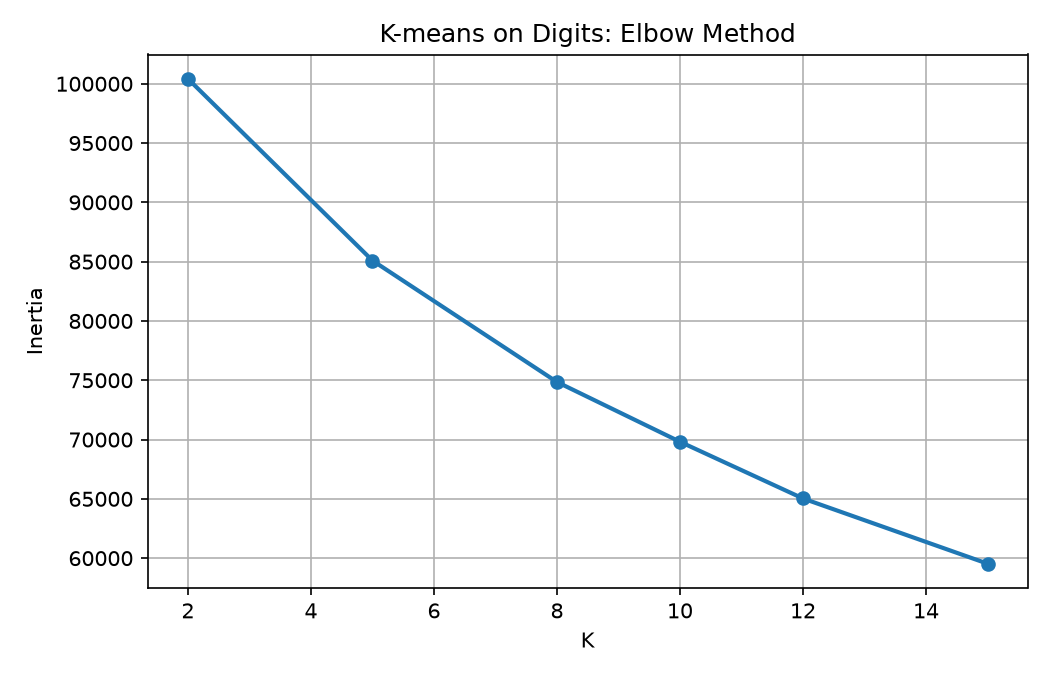
\includegraphics[width=0.68\textwidth]{exp10_elbow.png}\par
\small Fig. 1: Elbow method (inertia vs $K$).\par
\vspace{6pt}
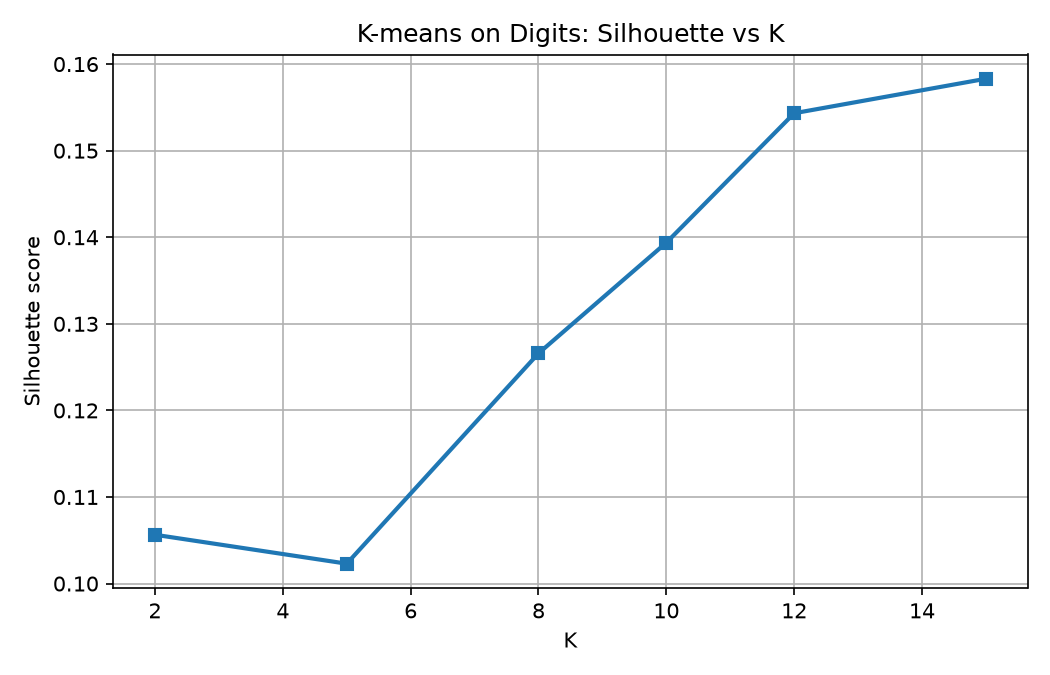
\includegraphics[width=0.68\textwidth]{exp10_sil.png}\par
\small Fig. 2: Silhouette score vs $K$ (best $K=15$).\par
\end{center}
\vspace{4pt}

\tooddpage
\expheading{RESULT}
\vspace{4pt}
{\fontsize{12}{15}\selectfont
The above program was implemented and executed successfully using Python, and the corresponding output was obtained and verified. The results of the \textbf{K-Means Clustering} were analyzed and found to be satisfactory, thereby achieving the desired objective of the experiment.\par
}

\vspace{12pt}

\noindent\textbf{Faculty Signature:} \underline{\hspace{3.6cm}} \hfill \textbf{Date:} \underline{\hspace{2.8cm}}\par

\tooddpage

% ============================================================
% EXPERIMENT 11
% ============================================================
{\makeatletter\let\vspace\@gobble\makeatother\fontsize{10}{11.4}\selectfont\setlength{\parskip}{0pt}\setlength{\abovedisplayskip}{0pt}\setlength{\belowdisplayskip}{0pt}
\begin{center}
\expheading{EXPERIMENT NO. 11}
\end{center}
\vspace{2pt}

\noindent\textbf{Date:} 30-10-2026\par
\vspace{6pt}

\expheading{TITLE}
\vspace{4pt}
\noindent Multilayer Feed-Forward Neural Network (MLP) on Wine Quality Dataset using Keras\par
\vspace{4pt}

\expheading{AIM}
\vspace{4pt}
\noindent To build and train a Multilayer Feed-Forward Neural Network (MLP) using Keras on the Wine Quality dataset and evaluate its classification performance. \par
\vspace{4pt}

\expheading{OBJECTIVE}
\vspace{2pt}
\fullrule
\vspace{4pt}
\noindent To implement an MLP using Keras for multi-class classification on the Wine Quality dataset, train it with backpropagation, and evaluate it using train and test accuracy with an accuracy versus epoch plot. \par
\vspace{4pt}

\expheading{THEORY}
\vspace{4pt}
A Multilayer Feed-Forward Neural Network consists of an input layer, one or more hidden layers and an output layer. Each neuron computes a weighted sum followed by a nonlinear activation:
\[a=\sigma\left(\sum_{j}w_jx_j+b\right)\]
The network is trained by backpropagation, which computes the gradients of the loss with respect to every weight using the chain rule and updates the weights by gradient descent:
\[w:=w-\eta\frac{\partial L}{\partial w}\]
For multi-class classification the output layer uses the softmax activation:
\[\text{softmax}(z_k)=\frac{e^{z_k}}{\sum_{j=1}^{K}e^{z_j}}\]
and the network is optimized using the categorical cross-entropy loss:
\[L=-\frac{1}{n}\sum_{i=1}^{n}\log\left(\hat{y}_{i,c_i}\right)\]
Keras is a high-level deep learning API used to define, compile and train the network.
\vspace{4pt}

\expheading{PROCEDURE}
\vspace{4pt}
\noindent 1. Load the Wine Quality dataset\par
\noindent\hspace*{0.55cm}Load the Wine Quality dataset using Pandas. Separate the input features (such as acidity, sugar, pH, alcohol, etc.) from the target variable, quality.\par
\noindent 2. Preprocess the data\par
\noindent\hspace*{0.55cm}Check for missing values and duplicate records, if any. Separate the dataset into input X and target y. Encode the quality labels appropriately for classification.\par
\noindent 3. Split the dataset\par
\noindent\hspace*{0.55cm}Divide the data into training and testing sets, for example, 80\% for training and 20\% for testing using train\_test\_split().\par
\noindent 4. Scale the input features\par
\noindent\hspace*{0.55cm}Apply feature scaling such as StandardScaler so that all input features have a comparable range. This helps the neural network converge faster during training.\par
\noindent 5. Design the MLP using Keras\par
\noindent\hspace*{0.55cm}Create a Keras Sequential model containing an input layer, one or more fully connected (Dense) hidden layers with ReLU activation, and an output layer with softmax activation. The network is 11 inputs $\rightarrow$ Dense(32, ReLU) $\rightarrow$ Dense(16, ReLU) $\rightarrow$ Dense(1, softmax)\par
\noindent 6. Compile the model\par
\noindent\hspace*{0.55cm}Compile the MLP using an optimizer such as Adam, an appropriate classification loss function such as categorical\_crossentropy, and accuracy as the evaluation metric.\par
\noindent 7. Train the network\par
\noindent\hspace*{0.55cm}Train the model using model.fit() for number of epochs=150 and batch size=100. During training, forward propagation calculates predictions, while backpropagation calculates gradients of the loss and updates the weights using the optimizer.\par
\noindent 8. Evaluate the trained model\par
\noindent\hspace*{0.55cm}Evaluate the model on the unseen test dataset using model.evaluate(). Record the test loss and test accuracy and compare the results of the different MLP architectures. \par
\vspace{4pt}

\expheading{DATASET DESCRIPTION}
\vspace{4pt}
\noindent Dataset Name: Wine Quality Dataset (Red Wine) \hspace{0.3cm} Source: winequality-red.csv (UCI)\par
\noindent Number of Samples: 1599 (1279 train / 320 test) \hspace{0.3cm} Number of Features: 11\par
\noindent Classes: 6 quality grades (3--8, reindexed 0--5)\par
\noindent Description: Physicochemical test results of red wine; the target is the sensory quality score. \par
\vspace{4pt}
} % end sheet-local tightening
\toevenpage
\expheading{PROGRAM}
\vspace{6pt}

\begin{lstlisting}
import os
os.environ.setdefault("KERAS_BACKEND", "torch")
import numpy as np
import pandas as pd
import matplotlib
matplotlib.use("Agg")
import matplotlib.pyplot as plt
import keras
from keras import layers
from sklearn.model_selection import train_test_split
from sklearn.preprocessing import StandardScaler
df = pd.read_csv("winequality-red.csv", sep=";")
print("Dataset:", df.shape)
print("Missing values:", int(df.isnull().sum().sum()))
print("Duplicates:", int(df.duplicated().sum()))
X = df.drop(columns=["quality"])
y = df["quality"] - 3
X_train, X_test, y_train, y_test = train_test_split(X, y, test_size=0.2, random_state=42, stratify=y)
print("Train:", len(X_train), " Test:", len(X_test))
scaler = StandardScaler()
X_train_s = scaler.fit_transform(X_train).astype("float32")
X_test_s = scaler.transform(X_test).astype("float32")
y_train = np.asarray(y_train)
y_test = np.asarray(y_test)
model = keras.Sequential([
    layers.Input(shape=(11,)),
    layers.Dense(32, activation="relu"),
    layers.Dense(16, activation="relu"),
    layers.Dense(6, activation="softmax"),
])
model.compile(optimizer="adam", loss="sparse_categorical_crossentropy", metrics=["accuracy"])
\end{lstlisting}

\toevenpage
\expheading{PROGRAM (continued)}
\vspace{6pt}

\begin{lstlisting}
history = model.fit(X_train_s, y_train, epochs=150, batch_size=100, validation_data=(X_test_s, y_test), verbose=0)
loss, acc = model.evaluate(X_test_s, y_test, verbose=0)
print(f"Train accuracy: {history.history['accuracy'][-1]:.4f}")
print(f"Test loss: {loss:.4f}")
print(f"Test accuracy: {acc:.4f}")
plt.figure(figsize=(7, 4.5))
plt.plot(history.history["accuracy"], label="train")
plt.plot(history.history["val_accuracy"], label="test")
plt.xlabel("Epoch")
plt.ylabel("Accuracy")
plt.title("MLP on Wine Quality: Accuracy")
plt.legend()
plt.grid(True)
plt.tight_layout()
plt.savefig("exp11_acc.png", dpi=150)
\end{lstlisting}
\toevenpage
\expheading{OUTPUT}
\vspace{2pt}
\noindent\rule{\textwidth}{0.5pt}\par
\vspace{4pt}
\begin{verbatim}
Dataset: (1599, 12)
Missing values: 0
Duplicates: 240
Train: 1279  Test: 320
Train accuracy: 0.6935
Test loss: 0.9831
Test accuracy: 0.6281
\end{verbatim}
\vspace{4pt}

\begin{center}
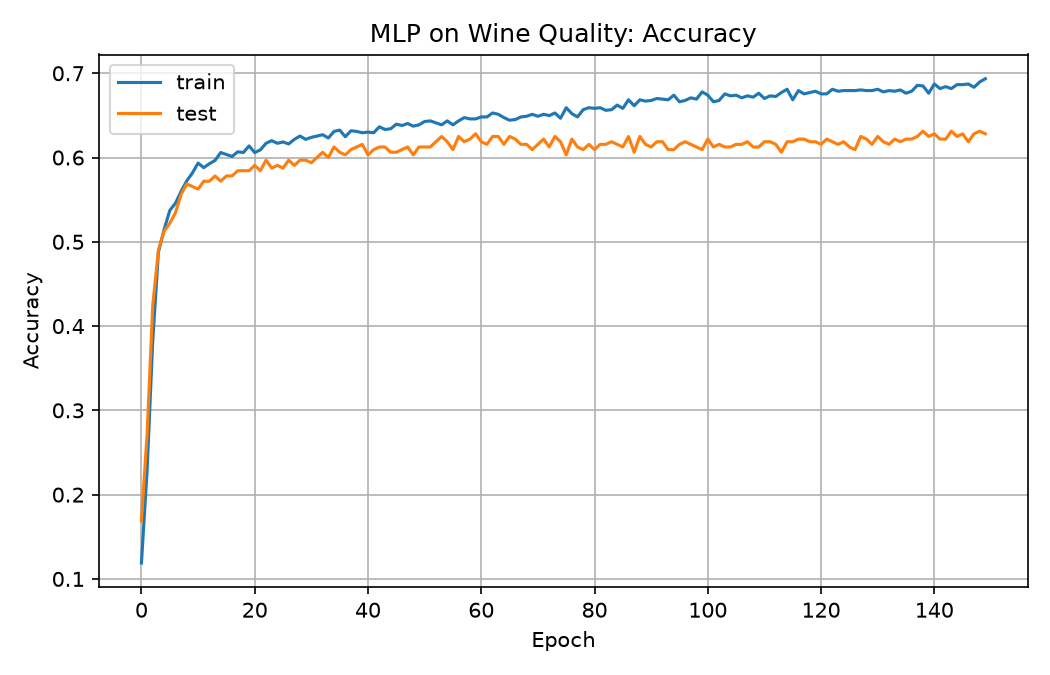
\includegraphics[width=0.72\textwidth]{exp11_acc.png}\par
\small Fig. 1: Training and test accuracy per epoch.\par
\end{center}
\vspace{4pt}

\tooddpage
\expheading{RESULT}
\vspace{4pt}
{\fontsize{12}{15}\selectfont
The above program was implemented and executed successfully using Python, and the corresponding output was obtained and verified. The results of the \textbf{Keras Multilayer Perceptron} were analyzed and found to be satisfactory, thereby achieving the desired objective of the experiment.\par
}

\vspace{12pt}

\noindent\textbf{Faculty Signature:} \underline{\hspace{3.6cm}} \hfill \textbf{Date:} \underline{\hspace{2.8cm}}\par

\end{document}

